% SPDX-License-Identifier: CC-BY-4.0
%
% Copyright (c) 2023 Nelson Vieira
%
% @author Nelson Vieira <nelson0.vieira@gmail.com>
% @license CC-BY-4.0 <https://creativecommons.org/licenses/by/4.0/legalcode.txt>
\section{An Application of the Theory}
\label{section:stage2}

This work proposes an application that gives users information about IoT
devices that inhabit their surroundings, like the type of information these devices
collect and what privacy options are available. This application is developed
for mobile phones due to the fact that these are the most used devices
and people take them everywhere they go, this is important because the application
uses georeferencing to show the location of the IoT devices. This application
has two main objectives, the first is to inform and educate users in order improve
their digital literacy on this particular field (privacy on IoT systems, and
IoT in general) and the other being to give users a way to make informed decisions
to protect their private data, in a concise and convenient place. Generally
the application will show the geolocation of the IoT devices, what type of
device it is, what type of data is being collect by the device. The application
will not detect the devices by itself, this will be done by the users themselves,
in the first iterations of the application it was discussed that the application
itself would automatically detect the devices by using some kind of sniffer
and would categorize what type of device it was and what type of data it
was collecting but it was discovered that this approach was too complex and
so it was not feasible to do with the constraints of this thesis. The application
is developed with Flutter, other options considered were React Native or a
progressive web application, but Flutter uses ahead of time and just in time
compilation, with Dart as it is programming language, while React Native uses
the Javascript programming language that was never created for mobile programming,
so it uses a bridge to convert Javascript to native components for Android
or iOS. Flutter has better performance and as such it was the chosen framework
for this application.

The first step before creating any prototypes or starting the development was
the creation of a software requirements specification
delineating the scope and vision for the application; the involved stakeholders;
containing contextual, data-flow and swimlane diagrams; software requirements, including
business, technology, functional and non-functional requirements; use cases
and requirements prioritisation.

% Types of data:
% Health
% Visual
% Audio
% Presence (if user is nearby)
% Location (precise location of user)
% Biometrics
% Environment
% Unique identification (with the help of other means)

% Information to be added to the app:
% What is the purpose of the data collection
% Who can access the data
% For how long is it stored
% Can the data identify anyone
% What is done with this data

% \section{Current Stage of the Work}

% The preliminary results of the study, based on 10 responses, show that everyone
% agrees that privacy is important to them and some people know that they
% should not share their personal information with anyone they do not trust
% (like clicking on random urls or using unprotected websites/software), but
% most of them think that privacy and security are the same concept, most
% respondents also do not read privacy notices but accept them to access the
% information they want to get to, most respondents use their devices mostly
% to access social networks and for work, when it comes to IoT, there is a
% dissonance between knowing the term and using devices like smart watches
% or RFID enabled devices, from the respondents that answered yes to using
% IoT devices most use because of work. It is also noted that most respondent
% have a background in engineering, so the responses are skewed. As a result,
% the survey will remain open to gather a larger number of responses and participants
% for more significant results and generalizations.

% \begin{table}[ht]
% \centering
% \begin{adjustbox}{width=0.5\textwidth}
% \small
% \noindent\begin{tabular}{p{0.17\textwidth}*{20}{|p{0.01\textwidth}}|}
% \hline
% \multicolumn{0}{|c|}{Work plan}
%     & \multicolumn{4}{c|}{January}
%     & \multicolumn{4}{c|}{February}
%     & \multicolumn{4}{c|}{March}
%     & \multicolumn{4}{c|}{April}
%     & \multicolumn{4}{c|}{May}
%     \\
% \hline
% \hline
% \multicolumn{0}{|l|}{Week}
%     & 1 & 2 & 3 & 4 & 1 & 2 & 3 & 4& 1 & 2 & 3 & 4& 1 & 2 & 3 & 4& 1 & 2 & 3 & 4 \\
% \hline
% % using the on macro to fill in twenty cells as `on'
% \multicolumn{0}{|l|}{Discovery and planning}
%     & \cellcolor[cmyk]{1,1,0,0}&&&& &&&& &&&& &&&&&&& \\
% \hline
% \multicolumn{0}{|l|}{Research enquiry}
%     & \cellcolor[cmyk]{1,1,0,0} & \cellcolor[cmyk]{1,1,0,0} & \cellcolor[cmyk]{1,1,0,0} & \cellcolor[cmyk]{1,1,0,0} & \cellcolor[cmyk]{1,1,0,0} & \cellcolor[cmyk]{1,1,0,0} & \cellcolor[cmyk]{1,1,0,0} & \cellcolor[cmyk]{1,1,0,0} & \cellcolor[cmyk]{1,1,0,0} & \cellcolor[cmyk]{1,1,0,0} & \cellcolor[cmyk]{1,1,0,0} & \cellcolor[cmyk]{1,1,0,0} &&&& &&&& \\
% \hline
% \multicolumn{0}{|l|}{State of the art}
%     & \cellcolor[cmyk]{1,1,0,0} & \cellcolor[cmyk]{1,1,0,0} & \cellcolor[cmyk]{1,1,0,0} & \cellcolor[cmyk]{1,1,0,0} & \cellcolor[cmyk]{1,1,0,0} & \cellcolor[cmyk]{1,1,0,0} & \cellcolor[cmyk]{1,1,0,0} & \cellcolor[cmyk]{1,1,0,0} &&&& &&&& &&&& \\
% \hline
% \multicolumn{0}{|l|}{Project requirements}
%     & \cellcolor[cmyk]{1,1,0,0} & \cellcolor[cmyk]{1,1,0,0} & \cellcolor[cmyk]{1,1,0,0} & \cellcolor[cmyk]{1,1,0,0} &&&& &&&& &&&& &&&& \\
% \hline
% \multicolumn{0}{|l|}{Wireframes and user stories}
%     &&&& & \cellcolor[cmyk]{1,1,0,0} & \cellcolor[cmyk]{1,1,0,0} & \cellcolor[cmyk]{1,1,0,0} & \cellcolor[cmyk]{1,1,0,0} &&&& &&&& &&&& \\
% \hline
% \multicolumn{0}{|l|}{Prototyping and refinement}
%     &&&&&& && \cellcolor[cmyk]{1,1,0,0} & \cellcolor[cmyk]{1,1,0,0} & \cellcolor[cmyk]{1,1,0,0} & \cellcolor[cmyk]{1,1,0,0} &&&& &&&& &  \\
% \hline
% \multicolumn{0}{|l|}{Development}
%     &&&& &&&& & \cellcolor[cmyk]{1,1,0,0} & \cellcolor[cmyk]{1,1,0,0} & \cellcolor[cmyk]{1,1,0,0} & \cellcolor[cmyk]{1,1,0,0} & \cellcolor[cmyk]{1,1,0,0} & \cellcolor[cmyk]{1,1,0,0} & \cellcolor[cmyk]{1,1,0,0} & \cellcolor[cmyk]{1,1,0,0} & \cellcolor[cmyk]{1,1,0,0} & \cellcolor[cmyk]{1,1,0,0} & \cellcolor[cmyk]{1,1,0,0} & \cellcolor[cmyk]{1,1,0,0} \\
% \hline
% \multicolumn{0}{|l|}{Tests and iterations}
%     &&&& &&&& &&& & \cellcolor[cmyk]{1,1,0,0} & \cellcolor[cmyk]{1,1,0,0} & \cellcolor[cmyk]{1,1,0,0} & \cellcolor[cmyk]{1,1,0,0} & \cellcolor[cmyk]{1,1,0,0} &&&&  \\
% \hline
% \multicolumn{0}{|l|}{Release and documentation}
%     &&&& &&&& &&&& &&&& & \cellcolor[cmyk]{1,1,0,0} & \cellcolor[cmyk]{1,1,0,0} & \cellcolor[cmyk]{1,1,0,0} & \cellcolor[cmyk]{1,1,0,0} \\
% \hline
% \end{tabular}
% \end{adjustbox}
% \vspace{1em}
% \caption{Work plan timeline}
% \label{workchart}
% \end{table}

% As can be seen in Table \ref{workchart}, the first months will involve the
% design of the application and the enquiry of the study followed by the development
% of the application and the synthesis of the study, and finally testing and
% refinement of the application. Because of the exploratory nature of this
% work the application might suffer alterations to the design, specially in
% the testing stage, and also depending on the results of the study.

\subsection{Software Requirements Specification}
\label{subsection:software_requirements}

A software requirements specification aims to define the details and principles
of the privacy assisting
IoT application with the ultimate goal of assisting in the development
of the application. It is a fundamental aspect of software development as it
helps developers understand what the project entails, from the tools that will be
used to knowing what features to implement, without this important first step projects
may fail due to incomplete or undefined requirements or succumb to feature creep.
Defining the scope of the project helps to understand
how to better implement the application.
Stakeholders tell us who communicates
with the system directly or indirectly. Business requirements are
defined in order to know in detail the possibilities of value for both sides.
The contextual diagram gives a general understanding of all actions between the
system and the active parties, the swimlane diagram provides a detailed
view of each step by the intervening parties in a specific scenario. The data
flow diagram explains in detail the outcomes of the specific actions. Finally,
the technology requirements enable an understanding of the project's budget and
the system's final design.

\subsubsection{Scope and Vision}

This application provides information about IoT devices in the users'
surroundings like the type of information
these devices collect and what privacy options are available. The main objective
of this application is to provide users with another option in order to protect
their private data. The application will show the geolocation of the IoT
devices, what type of device it is, what type of data is being collect by
the device. As for competition there are other similar
online systems with the same scope as this project. The application offers
an easier way to search for information about the IoT devices that are around users'
location.

\subsubsection{Stakeholders}

A stakeholder can be a person, group, or organisation that is involved in
the project, is affected by its process and outcome or can influence its
process and outcome. Stakeholders can be internal or external to the project
team and the organisation.

It is important to identify the stakeholders to make sure to get all the
right requirements for the project and to develop a system that can match
the proposed problem well.

The following stakeholders have been identified for this application:

\begin{itemize}
    \item[$\bullet$] \textbf{Software developer/Application administrator}: The programmers are the ones who create the application and even if they do not use it they are directly related to it.
    \item[$\bullet$] \textbf{IoT Device Owners}: These device owners are be priority stakeholders being that the application in good part will be directed to them, device owners have an indirect influence.
    \item[$\bullet$] \textbf{Application Users}: The users are be the main focus of this project, they are the ones that provide the information that will be inserted in the application, since they can change the course of the project they have a direct influence.
    \item[$\bullet$] \textbf{Thesis advisor}: Because this application is implemented in the context of a master's thesis, the advisor has an indirect influence during the implementation and the final product.
    \item[$\bullet$] \textbf{University of Madeira}: Because this application is implemented in the context of a master's thesis, the university as an organization has an indirect influence on the final product.
    \item[$\bullet$] \textbf{Legislation}: The legislation in relation to the privacy of the collected data allows to impose rules on the use of the data. It has an indirect influence.
\end{itemize}

\subsubsection{Contextual Diagram}

The contextual diagram aims to establish links between the system
and the other actors that interact with the application.

Identifies the identities external to the application that interact with
the system by exchanging data and control.
Figure \ref{fig:contextual diagram} represents the interaction between users, the
application administrator and the application itself.

\begin{figure}[H]
    \centering
    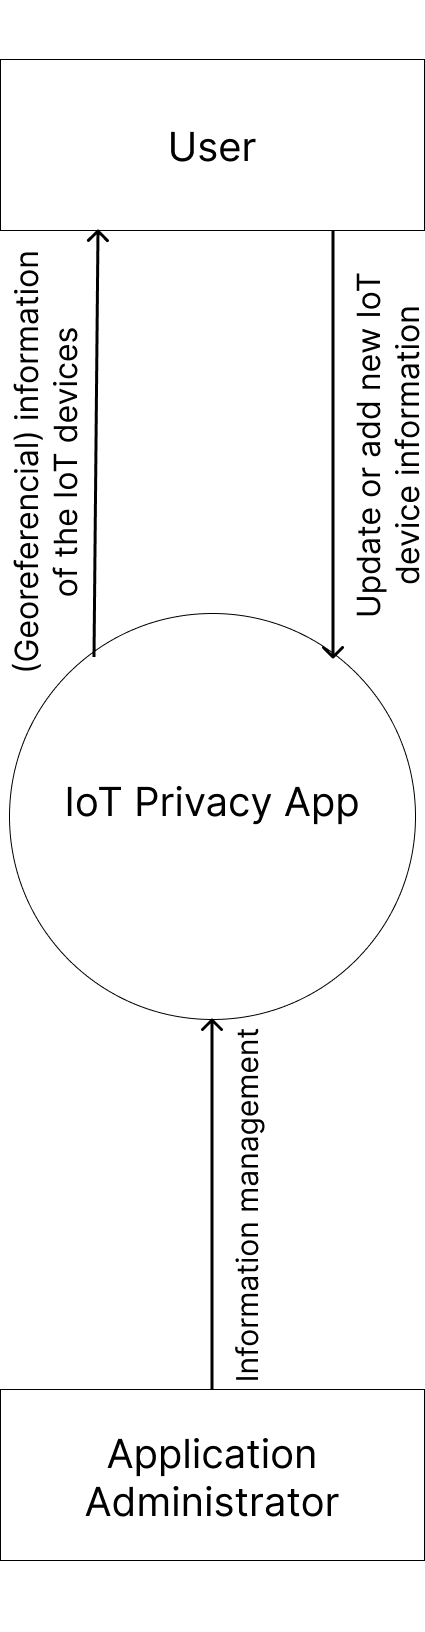
\includegraphics[width=3.5cm]{../app/docs/software_requirements/assets/images/contextual_diagram.png}
    \caption{Contextual diagram depicting the interaction between two stakeholders, the user and the administrator, and the application.}
    \label{fig:contextual diagram}
\end{figure}

The interaction links between the stakeholders and the application as represented
on the contextual diagram can be dissected as follows:\\
\newline
User: \\
\newline
→ Receives:

$\bullet$ (Georeferencial) information of the IoT devices\\
\newline
→ Sends:

$\bullet$ Update or addition of IoT device information\\
\newline
Application Administrator (Programmer): \\
\newline
→ Receives:

$\bullet$ All information related to the application\\
\newline
→ Sends:

$\bullet$ Information management

\subsubsection{Data Flow Diagram}

A data flow diagram shows how information flows between the various entities
in the system and their relationships.

\begin{figure}[H]
    \centering
    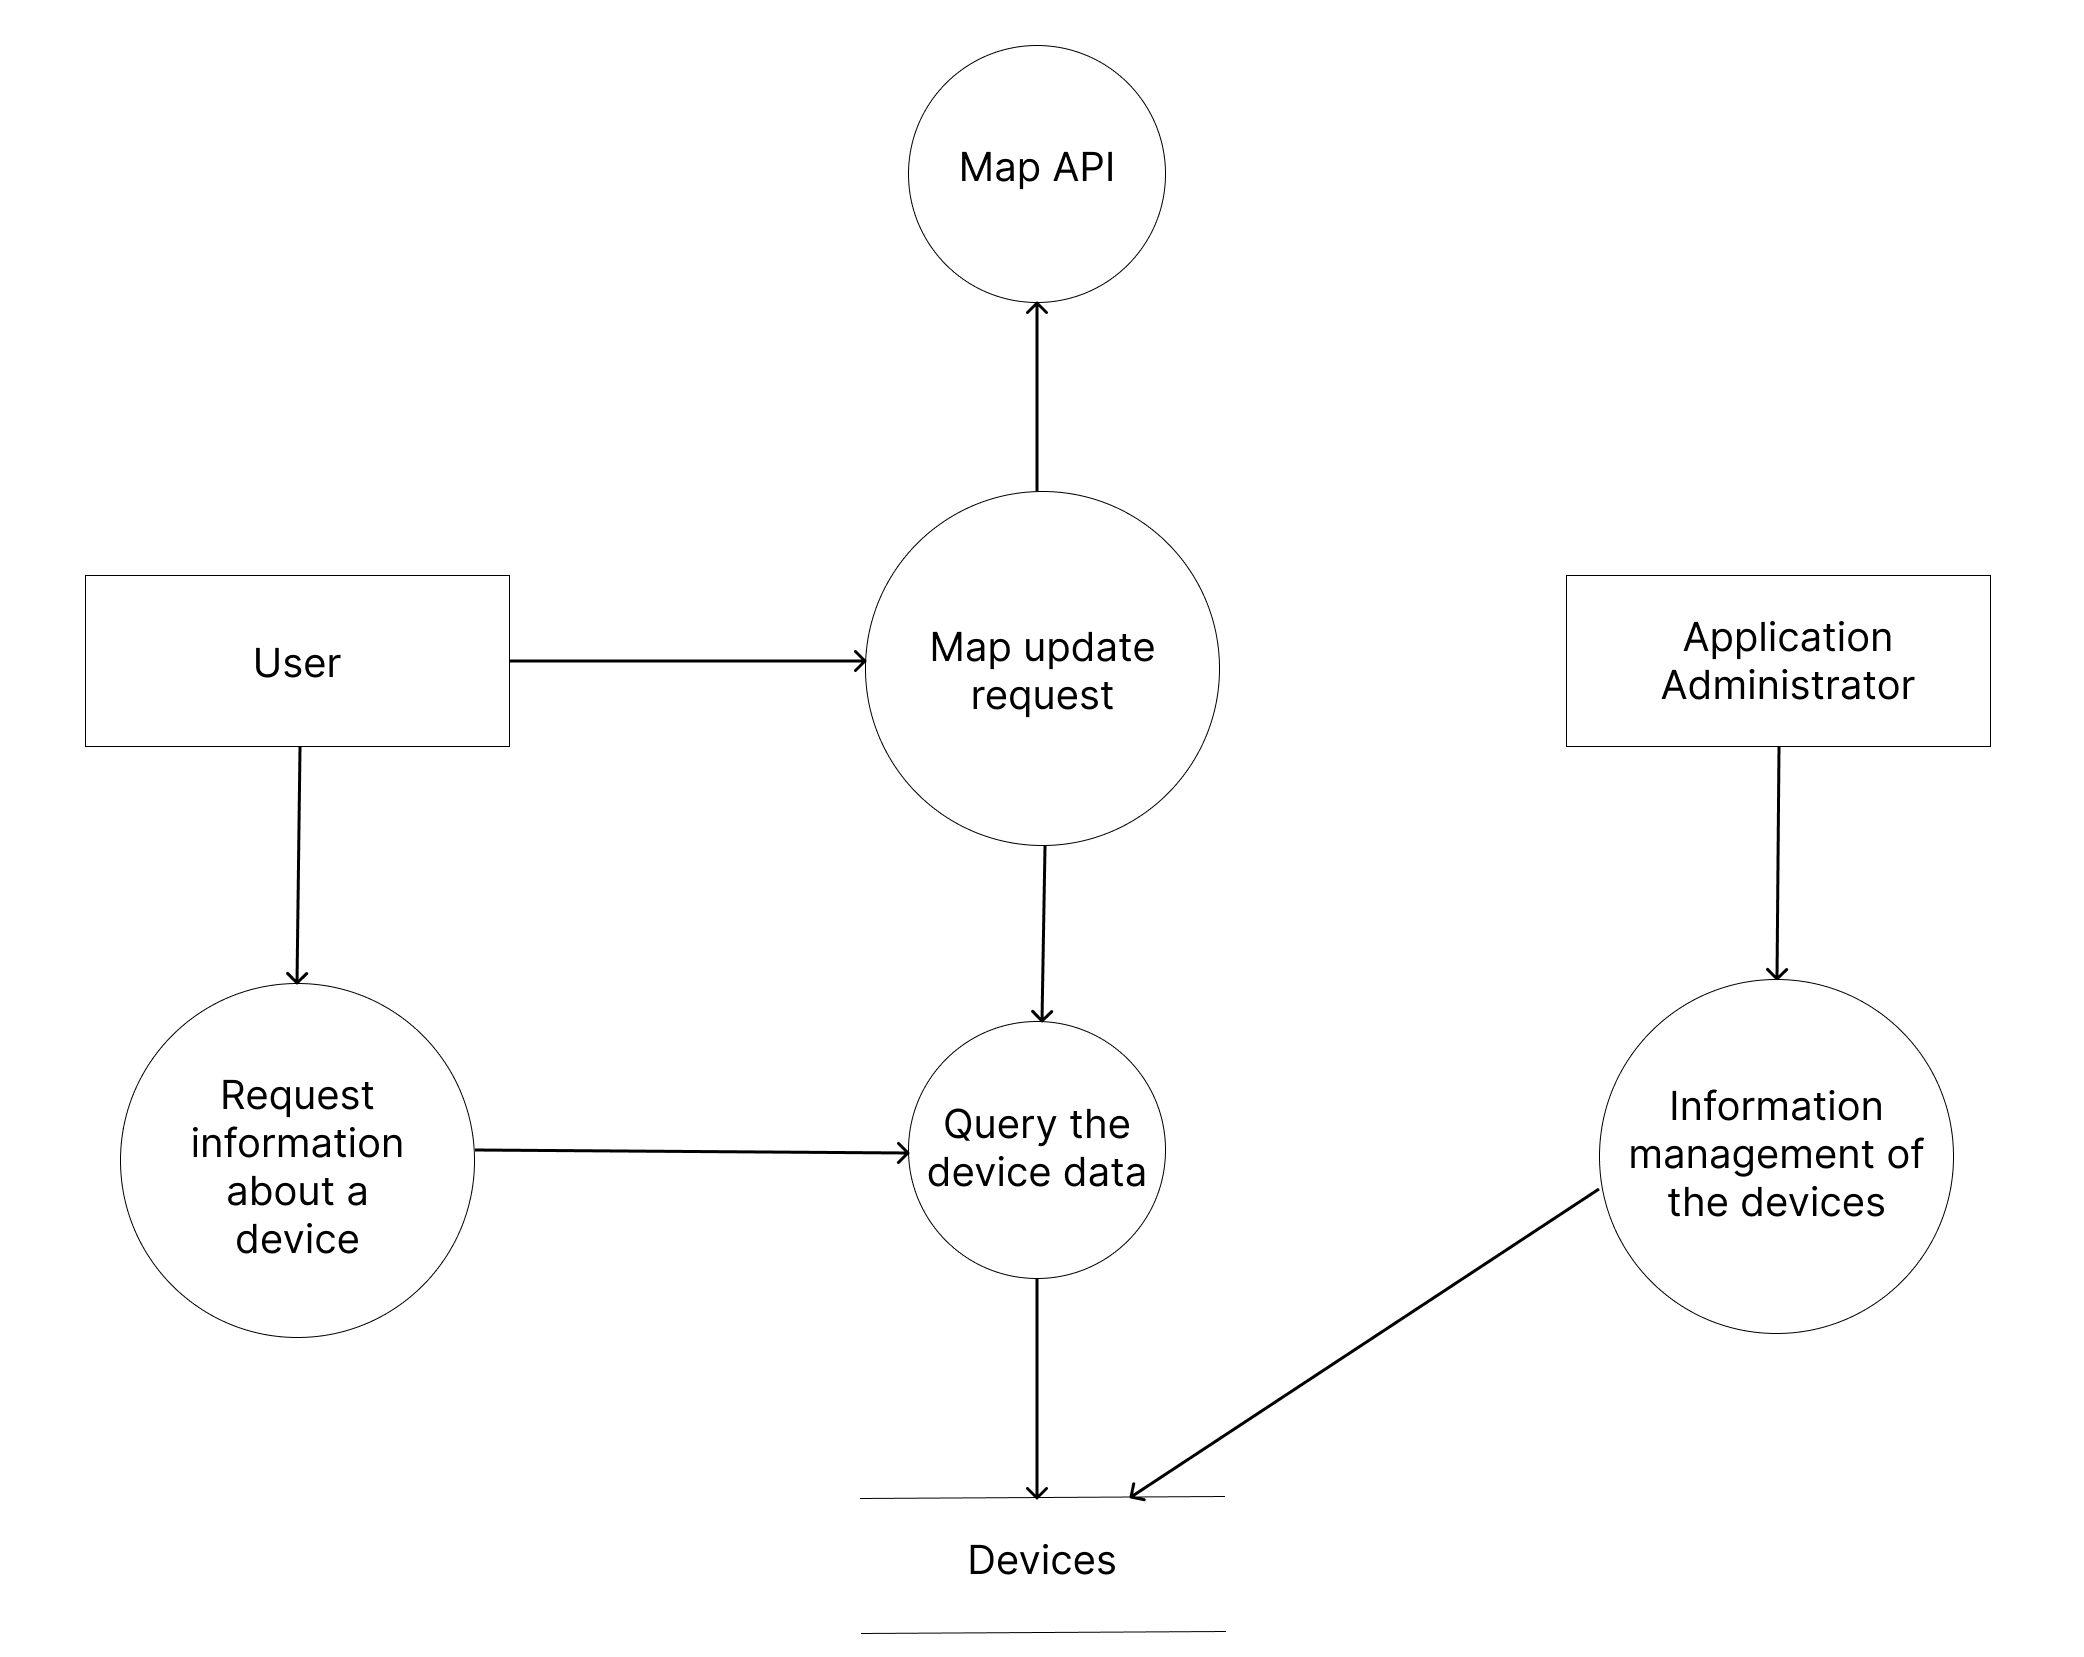
\includegraphics[width=15cm]{../app/docs/software_requirements/assets/images/data_flow_diagram.png}
    \caption{Data flow diagram.}
    \label{fig:data flow diagram}
\end{figure}

As shown in Figure \ref{fig:data flow diagram}, the user can browse the application
map, which will be interacted through an API,
and see the location of the IoT devices, the user can also look up information
about the devices by clicking on a device on the map or by searching for
the device in the application. The administrator of the application is responsible for
its maintenance by correcting or deleting incorrect data, implementing security
measures and for the stability and reliability of the system.

\subsubsection{Swimlane Diagram}

A swimlane diagram is a type of flowchart in which processes and decisions
are grouped into lanes. Parallel lines divide the diagram into lanes, each
lane being assigned to a stakeholder and the application.

\begin{figure}[H]
    \centering
    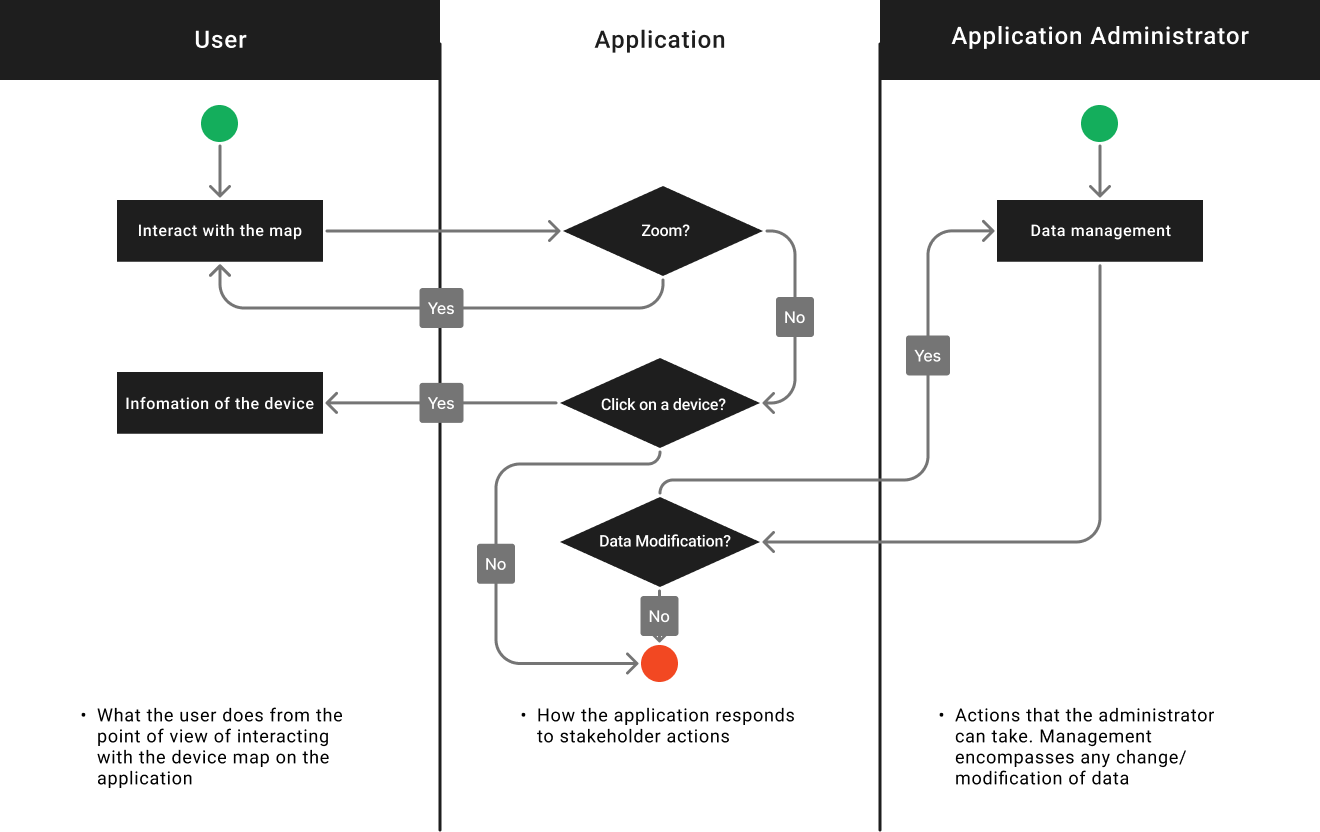
\includegraphics[width=15cm]{../app/docs/software_requirements/assets/images/swimlane_diagram.png}
    \caption{Swimlane diagram.}
    \label{fig:diagram swimlane}
\end{figure}

This swimlane diagram represents a high level view of a possible user interaction
from the application's map, in Figure \ref{fig:diagram swimlane} the user can view the location of
IoT devices and can see more information about a particular device by selecting
it on the map. The application administrator, as mentioned above, can modify the
devices' data.

\subsubsection{Business Requirements}

Business requirements describe in business terms what must be delivered
or achieved to deliver value. It is what defines the way of doing business,
reflecting the internal policy, the defined process and/or the basic rules
of conduct.  In other words, it is a set of instructions that users already
follow and that the system to be developed must contemplate. Restrictions,
validations, conditions and process exceptions are classic examples of business
rules. A business rule will not necessarily be reflected in the system as
a functionality, but it will certainly determine the behaviour of one or
more functionalities of the system.
\newline
No business requirements have been identified for this project.

\subsubsection{Technology Requirements}

Technology requirements describe what both hardware and software must be
used in order for a system to be realizable. In terms of hardware, it describes
what kind of physical components are needed for the software to work. The
software to be chosen must take into account the hardware that has been
chosen and what is intended by the stakeholders. This has implications for
how the system is implemented.
\newline
The technology requirements that have been identified for this project are as follows:
\begin{itemize}
    \item[$\bullet$] Firestore or similar database server
    \item[$\bullet$] Flutter framework with Dart being the main programming language
    \item[$\bullet$] Accessible on any smartphone (iOS or Android) \newline \textbf{Note}: There will not be a web based version available.
\end{itemize}
These requirements have been chosen so that the system is available to as
many users as possible regardless of the hardware they use. The database
will allow to store the information that the users provide about the IoT
devices. The application will be developed with Flutter since it uses ahead
of time and just in time compilation with Dart as its programming language.
Flutter has better performance than React Native or a PWA stack and as such it is the chosen framework for
this application.

\subsubsection{Requirements Table}

The requirements table identifies each feature and links each feature to an origin
which can come from brainstorming sessions or interviews for example.
This is important as it makes to managing requirements in the future easier.
Knowing where the requirements came from makes it simpler to clarify any questions
and refer back to the original source.
\newline
Table \ref{table:table1} lists all the features that have been identified, for
each feature it was identified the stakeholders to which it applies, a description
of the feature and its source. There have been identified 10 features that will
compose the backbone of the application.

\begin{longtable}{|l|p{0.2\textwidth}|p{0.2\textwidth}|p{0.4\textwidth}|p{0.15\textwidth}|}
    \hline
    \rowcolor{blue!5}
    \textbf{R\#} & \textbf{Feature} & \textbf{Applicable stakeholders} & \textbf{Description} & \textbf{Source} \\
    \hline
    \textbf{1} & Navigate the map & User & \textbf{User}: The system should allow the user to scroll through the map of devices & Dissertation preparation \\
    \hline
    \textbf{2} & Select device on the map & User & \textbf{User}: The system should allow the user to select a device on the map to view more information & Dissertation preparation \\
    \hline
    \textbf{3} & Query devices through parameters & User & \textbf{User}: The system should allow the user to consult devices of only a certain type, data collected, general location & Dissertation preparation \\
    \hline
    \textbf{4} & Query statistics of the devices & User & \textbf{User}: The system should allow consulting statistics of devices & Dissertation preparation \\
    \hline
    \textbf{5} & Add a device & User & \textbf{User}: The system should allow the user to add a new device with name, category, data collected, location, etc. & Dissertation preparation \\
    \hline
    \textbf{6} & Edit a device & User & \textbf{User}: The system should allow the user to change some data of a device & Dissertation preparation \\
    \hline
    \textbf{7} & Delete a device & App Administrator & \textbf{App Administrator}: The system should allow the administrator to delete a device & Dissertation preparation \\
    \hline
    \textbf{8} & Create account & User & \textbf{User}: The system shall allow a user to create an account. & Dissertation preparation \\
    \hline
    \textbf{9} & Select privacy choices & User & \textbf{User}: The system shall allow the user to select their privacy choices for a certain device if the device allows for it. & Dissertation preparation \\
    \hline
    \textbf{10} & See more information about privacy in IoT & User & \textbf{User}: The system shall allow the user to check what the terms used in the application mean. & Survey results \\
    \hline
    \caption{Requirements table.}
    \label{table:table1}
\end{longtable}

% \begin{table}[H]
%     \centering
%     \begin{adjustbox}{width=1\textwidth,center=\textwidth}
%     \begin{tabular}{|l|p{0.2\textwidth}|p{0.2\textwidth}|p{0.4\textwidth}|p{0.15\textwidth}|}
%         \hline
%         \rowcolor{blue!5}
%         \textbf{R\#} & \textbf{Feature} & \textbf{Applicable stakeholders} & \textbf{Description} & \textbf{Source} \\
%         \hline
%         \textbf{1} & Navigate the map & User & \textbf{User}: The system should allow the user to scroll through the map of devices & Dissertation preparation \\
%         \hline
%         \textbf{2} & Select device on the map & User & \textbf{User}: The system should allow the user to select a device on the map to view more information & Dissertation preparation \\
%         \hline
%         \textbf{3} & Query devices through parameters & User & \textbf{User}: The system should allow the user to consult devices of only a certain type, data collected, general location & Dissertation preparation \\
%         \hline
%         \textbf{4} & Query statistics of the devices & User & \textbf{User}: The system should allow consulting statistics of devices & Dissertation preparation \\
%         \hline
%         \textbf{5} & Add a device & User & \textbf{User}: The system should allow the user to add a new device with name, category, data collected, location, etc. & Dissertation preparation \\
%         \hline
%         \textbf{6} & Edit a device & User & \textbf{User}: The system should allow the user to change some data of a device & Dissertation preparation \\
%         \hline
%         \textbf{7} & Delete a device & App Administrator & \textbf{App Administrator}: The system should allow the administrator to delete a device & Dissertation preparation \\
%         \hline
%         \textbf{8} & Create account & User & \textbf{User}: The system shall allow a user to create an account. & Dissertation preparation \\
%         \hline
%         \textbf{9} & Select privacy choices & User & \textbf{User}: The system shall allow the user to select their privacy choices for a certain device if the device allows for it. & Dissertation preparation \\
%         \hline
%         \textbf{10} & See more information about privacy in IoT & User & \textbf{User}: The system shall allow the user to check what the terms used in the application mean. & Survey results \\
%         \hline
%     \end{tabular}
%     \end{adjustbox}
%     \vspace{1em}
%     \caption{Requirements table.}
%     \label{table:table1}
% \end{table}

\subsubsection{Functional Requirements}

Functional requirements \cite{fulton2017chapter} define the functions of a system or its components,
where functions are specifications or behaviours between system outputs and
inputs. These outline what developers must implement in order for users to
accomplish tasks, which then fulfil business requirements. Functional requirements are
essential to the success of a project.
After building the tracing table, the functional requirements that were needed
were extracted for each feature and grouped appropriately according to the
following groups:

\paragraph{User Requirements}

\textbf{UR1} - The system shall allow the user to navigate through the devices georeferences;
\newline
\textbf{UR2} - The system shall allow the user to select a device on the map to view more information;
\newline
\textbf{UR4} - The system shall allow the user to consult devices of only a certain category, data collected, etc.;
\newline
\textbf{UR5} - The system shall allow consulting statistics of the devices;
\newline
\textbf{UR6} - The system shall allow the user to create an account;
\newline
\textbf{UR7} - The system shall allow a logged in user to add a new device with name, category, data collected, location, etc.;
\newline
\textbf{UR8} - The system shall allow a logged in user to change associated data of a device;

\paragraph{Administrator Requirements}

\textbf{AR1} - The system shall allow a logged in administrator to add a new device with name, category, data collected, location, etc.;
\newline
\textbf{AR2} - The system shall allow a logged in administrator to change associated data of a device;
\newline
\textbf{AR3} - The system shall allow a logged in administrator to delete a device;

\paragraph{System Requirements}

\textbf{SR1} - The system shall generate statistics related to the IoT devices that reside in the database;

\subsubsection{Non-Functional Requirements}

\textbf{NFR1} - The system shall behave the same in different platforms (Android and iOS);

\subsubsection{Use Cases Diagram}

The use cases diagram \cite{wiegers2013software} provides a high level visualisation of the user
requirements. The box represents the system boundary. An actor's arrow
for a use case indicates that he is the primary actor for it.
The primary actor initiates the use case and derives the primary value
from it.

In Figure \ref{fig:use_cases_diagram}, it is possible to determine the use cases
that have been identified, based on the previously specified system requirements.
The use cases related to the user are: browsing the map, create an account, search for
a device, check device statistics, add and edit a device and consult information
about a specific device. Meanwhile the use cases for the application administrator are:
adding editing or deleting a device, although the administrator can do all other
tasks as a regular user.

\begin{figure}[H]
    \centering
    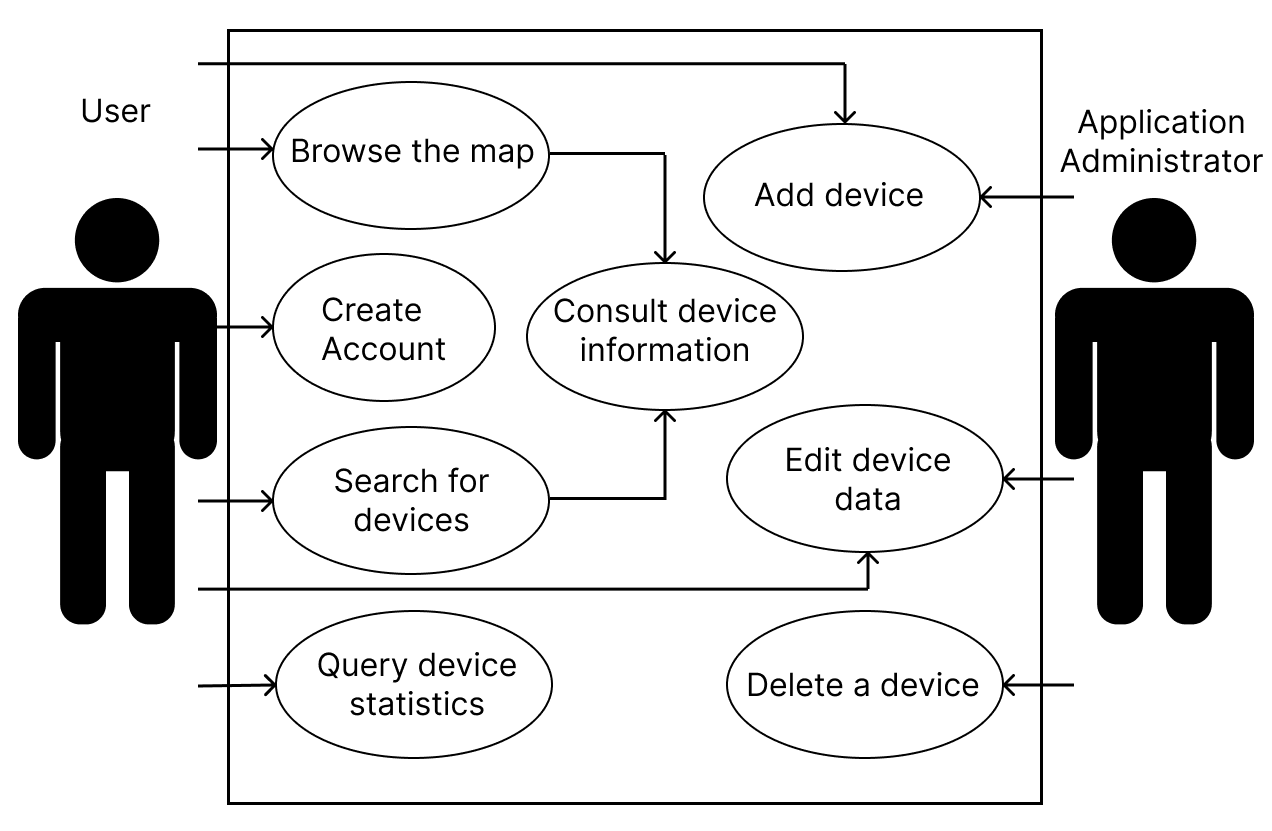
\includegraphics[width=15cm]{../app/docs/software_requirements/assets/images/use_cases_diagram.png}
    \caption{Use cases diagram.}
    \label{fig:use_cases_diagram}
\end{figure}

\subsubsection{Use Cases}

A use case is a type of classifier representing a
coherent functional unit provided by the system, subsystem, or class manifested
by sequences of interchangeable messages between systems and one or more
actors.

This technique describes the tasks that users need to perform with
the system or the user-system interaction that may be important to some
stakeholders. They also help in testing by checking that the functionality
has been implemented correctly. The use cases uses an Unified Modeling
Language (UML) notation.

Based on the use cases represented in Figure \ref{fig:use_cases_diagram},
use case ``Query devices through certain parameters'' has been detailed in Table \ref{table:use_case1};
use case ``Query device statistics'' has been detailed in Table \ref{table:use_case2};
use case ``Add a device'' has been detailed in Table \ref{table:use_case3};
use case ``Edit a device's data'' has been detailed in Table \ref{table:use_case4};
use case ``Delete a device'' has been detailed in Table \ref{table:use_case5};
and use case ``Create an account'' has been detailed in Table \ref{table:use_case6};

\begin{table}[H]
    \centering
    \begin{adjustbox}{width=1.2\textwidth,center=\textwidth}
        \begin{tabular}{|m{4cm}|m{12cm}|}
            \hline
            \textbf{ID and Name}: & UC-01 Query devices through certain parameters \\
            \hline
            \textbf{Created By}: & Nelson Vieira 20/02/2023 \\
            \hline
            \textbf{Primary Actor}: & End User \\
            \hline
            \textbf{Description}: & The user makes a device information query \\
            \hline
            \textbf{Trigger}: & The user wants to search device information \\
            \hline
            \textbf{Pre-conditions}: & N/A \\
            \hline
            \textbf{Post-conditions}: & POST-1. The user finds device information \\
            \hline
            \textbf{Normal Flow}: & \textbf{1.0 Query information of a device on the map}
            \begin{enumerate}
                \item The user browses the map
                \item The user clicks on the icon to show some information about the device
                \item The user clicks on the device pop-up
            \end{enumerate} \\
            \hline
            \textbf{Alternative Flow}: & \textbf{1.1 Device information search}
            \begin{enumerate}
                \item User enters device name
                \item The user chooses the device he wants from a list generated from the search performed
            \end{enumerate} \\
            \hline
            \textbf{Alternative Flow}: & \textbf{1.2 Alternative search for information from a device}
            \begin{enumerate}
                \item The user selects one of the parameters:
                \begin{enumerate}
                    \item Category
                    \item Name
                \end{enumerate}
                \item The user chooses the device he wants from a list generated from the search carried out
            \end{enumerate} \\
            \hline
            \textbf{Exceptions}: & \textbf{1.0.E1  The API is not working}
            \begin{enumerate}
                \item The system displays an alert message: ``We are having connection problems, please wait for a while''
            \end{enumerate} \\
            \hline
            \textbf{Priority}: & High \\
            \hline
            \textbf{Business Requirements}: & N/A \\
            \hline
            \textbf{Assumptions}: & N/A \\
            \hline
        \end{tabular}
    \end{adjustbox}
    \vspace{1em}
    \caption{Use case 1 - device information query.}
    \label{table:use_case1}
\end{table}

\begin{table}[H]
    \centering
    \begin{adjustbox}{width=1.2\textwidth,center=\textwidth}
        \begin{tabular}{|m{4cm}|m{12cm}|}
            \hline
            \textbf{ID and Name}: & UC-02 Device statistics query \\
            \hline
            \textbf{Created By}: & Nelson Vieira 20/02/2023 \\
            \hline
            \textbf{Primary Actor}: & End User \\
            \hline
            \textbf{Description}: & The user queries the statistics of the devices \\
            \hline
            \textbf{Trigger}: & The user wants to find statistics of devices \\
            \hline
            \textbf{Pre-conditions}: & N/A \\
            \hline
            \textbf{Post-conditions}: & POST-1. The system displays the statistics of the devices \\
            \hline
            \textbf{Normal Flow}: & \textbf{2.0 Device statistics query}
            \begin{enumerate}
                \item User selects statistics tab
                \item The user can only select certain parameters, such as:
                \begin{enumerate}
                    \item Category
                    \item Location
                \end{enumerate}
            \end{enumerate} \\
            \hline
            \textbf{Alternative Flow}: & N/A \\
            \hline
            \textbf{Exceptions}: & \textbf{2.0.E1  The API is not working}
            \begin{enumerate}
                \item The system displays an alert message: ``We are having connection problems, please wait for a while''
            \end{enumerate} \\
            \hline
            \textbf{Priority}: & Medium \\
            \hline
            \textbf{Business Requirements}: & N/A \\
            \hline
            \textbf{Assumptions}: & N/A \\
            \hline
        \end{tabular}
    \end{adjustbox}
    \vspace{1em}
    \caption{Use case 2 - statistics query.}
    \label{table:use_case2}
\end{table}

\begin{table}[H]
    \centering
    \begin{adjustbox}{width=1.15\textwidth,center=\textwidth}
        \begin{tabular}{|m{4cm}|m{12cm}|}
            \hline
            \textbf{ID and Name}: & UC-03 Add a device \\
            \hline
            \textbf{Created By}: & Nelson Vieira 22/02/2023 \\
            \hline
            \textbf{Primary Actor}: & End User \\
            \hline
            \textbf{Description}: & Addition of a new IoT device in the application \\
            \hline
            \textbf{Trigger}: & The user wants to add a new IoT device \\
            \hline
            \textbf{Pre-conditions}: & N/A \\
            \hline
            \textbf{Post-conditions}: & POST-1. A new IoT device is added to the application \\
            \hline
            \textbf{Normal Flow}: & \textbf{3.0 Add a device}
            \begin{enumerate}
                \item The user enters the following data of a new IoT device:
                \begin{enumerate}
                    \item Name
                    \item Type of data collected
                    \item Category
                    \item Photos
                \end{enumerate}
                \item The user clicks submit
                \item The user adds the location of the IoT device on the map
            \end{enumerate} \\
            \hline
            \textbf{Alternative Flow}: & N/A \\
            \hline
            \textbf{Exceptions}: & \textbf{3.0.E1  The device is already in the database}
            \begin{enumerate}
                \item The system displays an error message
            \end{enumerate} \\
            \hline
            \textbf{Priority}: & High \\
            \hline
            \textbf{Business Requirements}: & N/A \\
            \hline
            \textbf{Assumptions}: & N/A \\
            \hline
        \end{tabular}
    \end{adjustbox}
    \vspace{1em}
    \caption{Use case 3 - add a device.}
    \label{table:use_case3}
\end{table}

\begin{table}[H]
    \centering
    \begin{adjustbox}{width=1.1\textwidth,center=\textwidth}
        \begin{tabular}{|m{4cm}|m{12cm}|}
            \hline
            \textbf{ID and Name}: & UC-04 Edit a device's data \\
            \hline
            \textbf{Created By}: & Nelson Vieira 22/02/2023 \\
            \hline
            \textbf{Primary Actor}: & End User \\
            \hline
            \textbf{Description}: & Editing the data of an IoT device in the application \\
            \hline
            \textbf{Trigger}: & The user wants to edit an IoT device's data \\
            \hline
            \textbf{Pre-conditions}: & N/A \\
            \hline
            \textbf{Post-conditions}: & POST-1. The data that has been changed appears in the application \\
            \hline
            \textbf{Normal Flow}: & \textbf{4.0 Edit a device's data}
            \begin{enumerate}
                \item The user can change any of the following device data:
                \begin{enumerate}
                    \item Name
                    \item Category
                    \item Photos
                \end{enumerate}
                \item The user clicks on submit
            \end{enumerate} \\
            \hline
            \textbf{Alternative Flow}: & N/A \\
            \hline
            \textbf{Exceptions}: &
            % Exceptions: & \textbf{4.0.E1  Unique data already registered}
            % \begin{enumerate}
            %     \item The system displays an error message
            %     \item The system asks the user to enter different data
            % \end{enumerate}
            \textbf{4.0.E1  The device to be edited has been deleted in the meantime}
            \begin{enumerate}
                \item The system displays an error message
                \item The system prohibits editing
            \end{enumerate} \\
            \hline
            \textbf{Priority}: & High \\
            \hline
            \textbf{Business Requirements}: & N/A \\
            \hline
            \textbf{Assumptions}: & N/A \\
            \hline
        \end{tabular}
    \end{adjustbox}
    \vspace{1em}
    \caption{Use case 4 - edit a device's data.}
    \label{table:use_case4}
\end{table}

\begin{table}[H]
    \centering
    \begin{adjustbox}{width=1.2\textwidth,center=\textwidth}
        \begin{tabular}{|m{4cm}|m{12cm}|}
            \hline
            \textbf{ID and Name}: & UC-05 Delete a device \\
            \hline
            \textbf{Created By}: & Nelson Vieira 22/02/2023 \\
            \hline
            \textbf{Primary Actor}: & App Administrator \\
            \hline
            \textbf{Description}: & Deleting a device in the application \\
            \hline
            \textbf{Trigger}: & The administrator wants to delete a device \\
            \hline
            \textbf{Pre-conditions}: & PRE-1. The device to be deleted must be in the application's database \\
            \hline
            \textbf{Post-conditions}: & POST-1. The device is deleted from the application \\
            \hline
            \textbf{Normal Flow}: & \textbf{5.0 Delete a device}
            \begin{enumerate}
                \item The administrator deletes a device, through:
                \begin{enumerate}
                    \item ID of device
                    \item Name of device
                \end{enumerate}
                \item The administrator confirms the deletion
                \item The system deletes the device
            \end{enumerate} \\
            \hline
            \textbf{Alternative Flow}: & N/A \\
            \hline
            \textbf{Exceptions}: & \textbf{5.0.E1  The device to be deleted no longer exists in the database}
            \begin{enumerate}
                \item The system displays an error message
                \item The system prohibits deletion
            \end{enumerate} \\
            \hline
            \textbf{Priority}: & High \\
            \hline
            \textbf{Business Requirements}: & N/A \\
            \hline
            \textbf{Assumptions}: & It is assumed that the administrator has database access \\
            \hline
        \end{tabular}
    \end{adjustbox}
    \vspace{1em}
    \caption{Use case 5 - delete a device.}
    \label{table:use_case5}
\end{table}

\begin{table}[H]
    \centering
    \begin{adjustbox}{width=1.2\textwidth,center=\textwidth}
        \begin{tabular}{|m{4cm}|m{12cm}|}
            \hline
            \textbf{ID and Name}: & UC-06 Create an account \\
            \hline
            \textbf{Created By}: & Nelson Vieira 22/02/2023 \\
            \hline
            \textbf{Primary Actor}: & End User \\
            \hline
            \textbf{Description}: & Create a new end user account \\
            \hline
            \textbf{Trigger}: & The user wants to create an account \\
            \hline
            \textbf{Pre-conditions}: & PRE-1. The user wants to add a new device \\
            \hline
            \textbf{Post-conditions}: & POST-1. The account is created in the application \\
            \hline
            \textbf{Normal Flow}: & \textbf{6.0 Account creation process}
            \begin{enumerate}
                \item The user enter the following data in the register screen:
                \begin{enumerate}
                    \item Username
                    \item Email
                    \item Password
                \end{enumerate}
                \item The system adds the account data to the database
                \item An account confirmation email is sent to the email provided by the user
                \item The user confirms the account
            \end{enumerate} \\
            \hline
            \textbf{Alternative Flow}: & N/A \\
            \hline
            \textbf{Exceptions}: & \textbf{6.0.E1  The username already exists in the database}
            \begin{enumerate}
                \item The system displays an error message
                \item The system allows the user to recover the account
            \end{enumerate}
            \textbf{6.0.E2 The email already exists in the database}
            \begin{enumerate}
                \item The system displays an error message
                \item The system allows the user to recover the account
            \end{enumerate} \\
            \hline
            \textbf{Priority}: & High \\
            \hline
            \textbf{Business Requirements}: & N/A \\
            \hline
            \textbf{Assumptions}: & N/A \\
            \hline
        \end{tabular}
    \end{adjustbox}
    \vspace{1em}
    \caption{Use case 6 - create an account.}
    \label{table:use_case6}
\end{table}

\vspace*{\fill}

\subsubsection{Requirements Prioritisation}

Regarding the prioritization of requirements, the Quality Function Deployment technique
proposed by Cohen in 1995 \cite{cohen1995quality} is used to estimate the priority of a group of requirements.
This is based on the benefit of including a feature/requirement, the penalty of not including
it, and also the cost and risks associated with implementation. By using the MoSCoW method \cite{clegg1994case} the
initial features are reduced to facilitate the use of the Quality Function Deployment table.

In this approach, Table \ref{table:tabela moscow}, the values 0 and 1 are used. In case of 1 it means that the column requirement/feature
is a higher priority than the row one and if it is 0 the opposite is true.

\begin{table}[H]
    \centering
    \begin{adjustbox}{width=0.8\textwidth,center=\textwidth}
        \begin{tabular}{|>{\columncolor{gray!5!white}}r|r|r|r|r|r|r|r|r|r|r|}
            \hline
            \rowcolor{gray!5!white}
            & \textbf{R\#1} & \textbf{R\#2} & \textbf{R\#3} & \textbf{R\#4} & \textbf{R\#5} & \textbf{R\#6} & \textbf{R\#7} & \textbf{R\#8} & \textbf{R\#9} & \textbf{R\#10} \\
            \hline
            \textbf{R\#1} && 0 & 0 & 0 & 1 & 0 & 0 & 0 & 0 & 0 \\
            \hline
            \textbf{R\#2} & 1 && 0 & 0 & 1 & 0 & 0 & 0 & 0 & 0 \\
            \hline
            \textbf{R\#3} & 1 & 1 && 0 & 1 & 0 & 0 & 0 & 0 & 0 \\
            \hline
            \textbf{R\#4} & 1 & 1 & 1 && 1 & 0 & 0 & 0 & 1 & 1 \\
            \hline
            \textbf{R\#5} & 0 & 0 & 0 & 0 && 0 & 0 & 1 & 1 & 1 \\
            \hline
            \textbf{R\#6} & 1 & 1 & 1 & 1 & 1 && 0 & 0 & 1 & 1 \\
            \hline
            \textbf{R\#7} & 1 & 1 & 1 & 1 & 1 & 1 && 1 & 1 & 1 \\
            \hline
            \textbf{R\#8} & 1 & 1 & 1 & 1 & 0 & 1 & 0 && 1 & 1 \\
            \hline
            \textbf{R\#9} & 1 & 1 & 1 & 0 & 0 & 0 & 0 & 0 && 1 \\
            \hline
            \textbf{R\#10} & 1 & 1 & 1 & 0 & 0 & 0 & 0 & 0 & 0 & \\
            \hline
            \rowcolor{gray!20}
            \textbf{Total} & 8 & 7 & 6 & 3 & 6 & 2 & 0 & 2 & 5 & 6 \\
            \hline
        \end{tabular}
    \end{adjustbox}
    \vspace{1em}
    \caption{Prioritisation table using the MoSCoW technique.}
    \label{table:tabela moscow}
\end{table}

After this initial selection, the prioritisation of requirements was estimated, as shown in Table \ref{table:prioritisation table},
where it is ranked, on a scale of 1 to 9, the benefit and penalty
of each requirement. The cost and implementation risk associated to each feature is
also estimated.

\begin{landscape}
    \vspace*{\fill}
    \begin{table}[H]
        \centering
        \begin{adjustbox}{width=1.8\textwidth,center=\textwidth}
            \begin{tabular}{|>{\columncolor{gray!10!white}}r|r|r|r|r|r|r|r|r|r|r|}
                \hline
                \rowcolor{gray!10!white}
                \multicolumn{2}{|c|}{\textbf{Feature}} & \textbf{Relative benefit} & \textbf{Relative penalty} & \textbf{Total value} & \textbf{Value \%} & \textbf{Relative cost} & \textbf{Cost \%} & \textbf{Relative risk} & \textbf{Risk \%} & \textbf{Priority} \\
                \hline
                Navigate the map & 1 & 9 & 9 & 27 & 13,24 & 5 & 10,42 & 5 & 10,00 & 0,65 \\
                \hline
                Select device on the map & 2 & 9 & 9 & 27 & 13,24 & 5 & 10,42 & 5 & 10,00 & 0,65 \\
                \hline
                Add a device & 5 & 9 & 9 & 27 & 13,24 & 3 & 6,25 & 4 & 8,00 & 0,93 \\
                \hline
                See more information about privacy in IoT & 10 & 5 & 6 & 24 & 11,76 & 6 & 12,50 & 2 & 4,00 & 0,71 \\
                \hline
                Query devices through parameters & 3 & 6 & 8 & 20 & 9,80 & 7 & 14,58 & 6 & 12,00 & 0,37 \\
                \hline
                Select privacy choices & 9 & 5 & 7 & 19 & 9,31 & 6 & 12,50 & 8 & 16,00 & 0,33 \\
                \hline
                Query statistics of the devices & 4 & 3 & 5 & 11 & 5,39 & 5 & 10,42 & 7 & 14,00 & 0,22 \\
                \hline
                Create account & 8 & 8 & 9 & 15 & 7,35 & 5 & 10,42 & 5 & 10,00 & 0,36 \\
                \hline
                Edit a device & 6 & 7 & 8 & 22 & 10,78 & 3 & 6,25 & 4 & 8,00 & 0,76 \\
                \hline
                Delete a device & 7 & 4 & 4 & 12 & 5,88 & 3 & 6,25 & 4 & 8,00 & 0,41 \\
                \hline
                \rowcolor{gray!40}
                \multicolumn{2}{|c|}{\textbf{Total}} & 67 & 62 & \textbf{198} & 100,00 & \textbf{39} & 100,00 & \textbf{37} & 100,00 & \\
                \hline
            \end{tabular}
        \end{adjustbox}
        \vspace{1em}
        \caption{Features prioritisation table.}
        \label{table:prioritisation table}
    \end{table}
    \vspace*{\fill}
\end{landscape}

Using this method it is possible to get the requirements sorted by priority,
as seen in Table \ref{table:sorted requirements}.

\begin{table}[H]
    \centering
    \begin{adjustbox}{width=0.8\textwidth,center=\textwidth}
        \begin{tabular}{|c|c|c|c|}
            \hline
            \rowcolor{gray!5}
            \textbf{Rank} & \textbf{Feature} & \textbf{\# Feature} & \textbf{Priority} \\
            \hline
            1 & Add a device & 5 & 0,93 \\
            \hline
            2 & Edit a device & 6 & 0,76 \\
            \hline
            3 & See more information about privacy in IoT & 10 & 0,71 \\
            \hline
            4 & Navigate the map & 1 & 0,65 \\
            \hline
            5 & Select device on the map & 2 & 0,65 \\
            \hline
            6 & Delete a device & 7 & 0,41 \\
            \hline
            7 & Query devices through parameters & 3 & 0,37 \\
            \hline
            8 & Create an account & 8 & 0,36 \\
            \hline
            9 & Select privacy choices & 9 & 0,33 \\
            \hline
            10 & Query statistics of the devices & 4 & 0,22 \\
            \hline
        \end{tabular}
    \end{adjustbox}
    \vspace{1em}
    \caption{Highest priority requirements ordered.}
    \label{table:sorted requirements}
\end{table}

\subsubsection{Acceptance Criteria}

To make it easier to test whether the highest priority features that were chosen
previously were well implemented, these acceptance criteria were created for each
of them. These criteria help us understand the minimum conditions for this
application to be considered an MVP, i.e., for this project to have the minimum
possible requirements in order for it to be considered production ready.
\newline
For these acceptance criteria, the following was considered:

\begin{itemize}
    \item[$\bullet$] High-level functionality that must be present for the system to be usable
    \item[$\bullet$] Non-functional criteria and quality metrics that have to be satisfied
    \item[$\bullet$] Possibility of open problems or defects (we can guarantee that no defects or TBD is present for the system to be accepted)
    \item[$\bullet$] Legal or contractual restrictions (that have to be met for the system to be accepted)
\end{itemize}

\paragraph{Features}

\begin{itemize}
    \item[$\bullet$] Add a device
        \begin{itemize}
            \item[$\circ$] The system allows the user to add a new device that is not yet present in the database
        \end{itemize}
    \item[$\bullet$] Edit a device
    \begin{itemize}
        \item[$\circ$] The system allows the editing of an existing device
        \item[$\circ$] The system saves in the database the changes that have been made
    \end{itemize}
    \item[$\bullet$] Delete a device
    \begin{itemize}
        \item[$\circ$] The system allows the deletion of an existing device
        \item[$\circ$] The system deletes the device from its database
    \end{itemize}
    \item[$\bullet$] Navigate the map
    \begin{itemize}
        \item[$\circ$] The system can represent the devices on the map
        \item[$\circ$] The system allows the user to navigate throughout the map and view the devices
    \end{itemize}
    \item[$\bullet$] Query devices through parameters
    \begin{itemize}
        \item[$\circ$] The system allows searching devices by the certain parameters like the category, the type of data collected
    \end{itemize}
    \item[$\bullet$] Select device on map
    \begin{itemize}
        \item[$\circ$] The system allows the user to select a device on the map
    \end{itemize}
    \item[$\bullet$] See more information about privacy in IoT
    \begin{itemize}
        \item[$\circ$] The system allows the user to see more information about privacy in IoT
    \end{itemize}
    \item[$\bullet$] Select privacy choices
    \begin{itemize}
        \item[$\circ$] The system allows the user to select a device and view its details
        \item[$\circ$] The system allows the user to select privacy choices for that device (if that option is available)
    \end{itemize}
    \item[$\bullet$] Consult devices' statistics
    \begin{itemize}
        \item[$\circ$] The system allows the user to consult statistics concerning the devices
    \end{itemize}
    \item[$\bullet$] Create account
    \begin{itemize}
        \item[$\circ$] The system allows the creation of an account
        \item[$\circ$] The user has to enter its username, email and a password
        \item[$\circ$] The system can detect whether the email is already in use
        \item[$\circ$] The system can send a profile creation confirmation email
        \item[$\circ$] The user can confirm the profile creation
        \item[$\circ$] The system allows the user to sign in
    \end{itemize}
\end{itemize}

\subsection{Prototype}

After creating the software requirements specification, the prototypes were
created. For the creation of the prototypes the following tools were used: Figma
and GIMP. Figma was the primary tool for the design while GIMP was mostly used
for image manipulation as it is a more specialized software tool.

At first a low level prototype was made in order to understand the
general design and user interaction of the application. Figure \ref{fig:lowlevelprototype}
shows tree pages of the low level prototype, these being the homepage, about
and faq pages. This is a rough sketch, there are barely any details added to each page,
this only serves to get a general idea of where icons and other items
will be placed and how the navigation between screens will work.

\begin{figure}
    \centering
    \begin{subfigure}{0.33\textwidth}
        \centering
        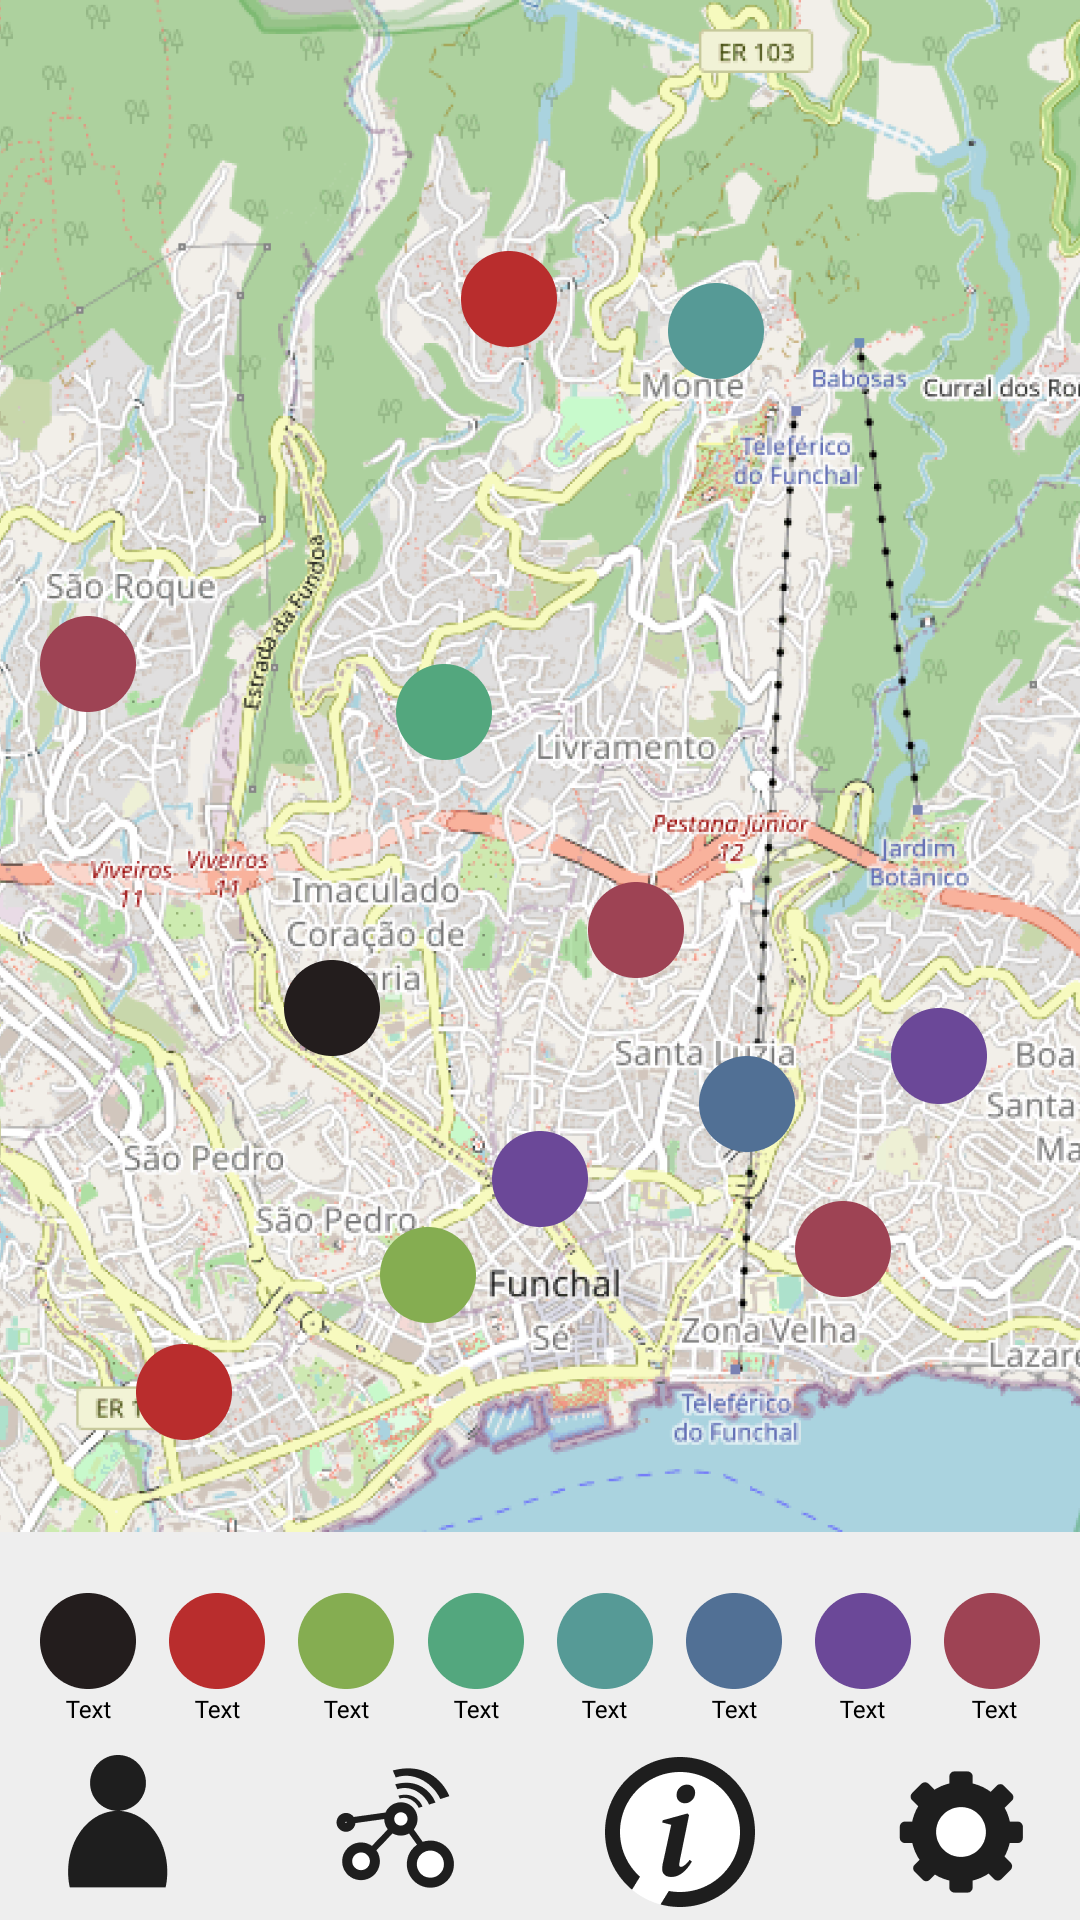
\includegraphics[width=130pt]{../assets/images/low_homepage.png}
        \caption{}
        \label{fig:lowhome}
    \end{subfigure}%
    \begin{subfigure}{0.33\textwidth}
        \centering
        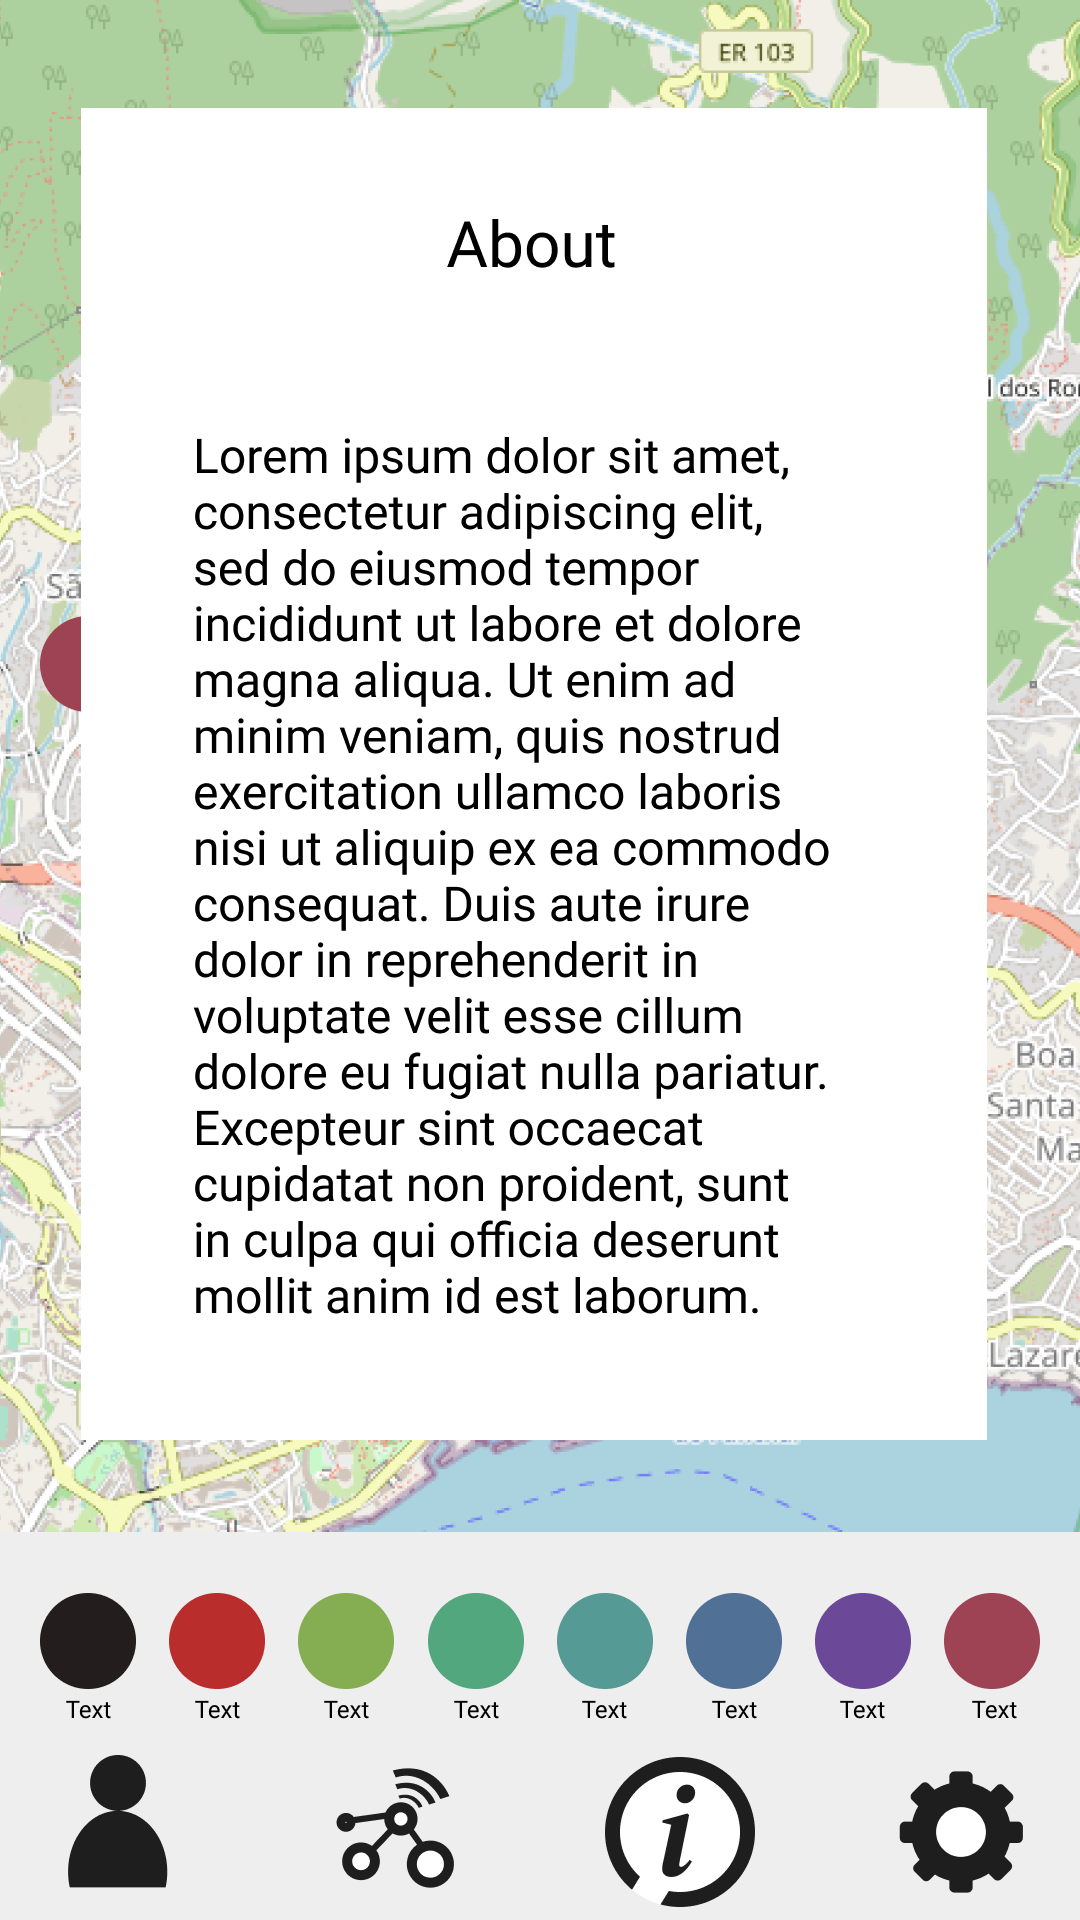
\includegraphics[width=130pt]{../assets/images/low_about.png}
        \caption{}
        \label{fig:lowabout}
    \end{subfigure}%
    \begin{subfigure}{0.33\textwidth}
        \centering
        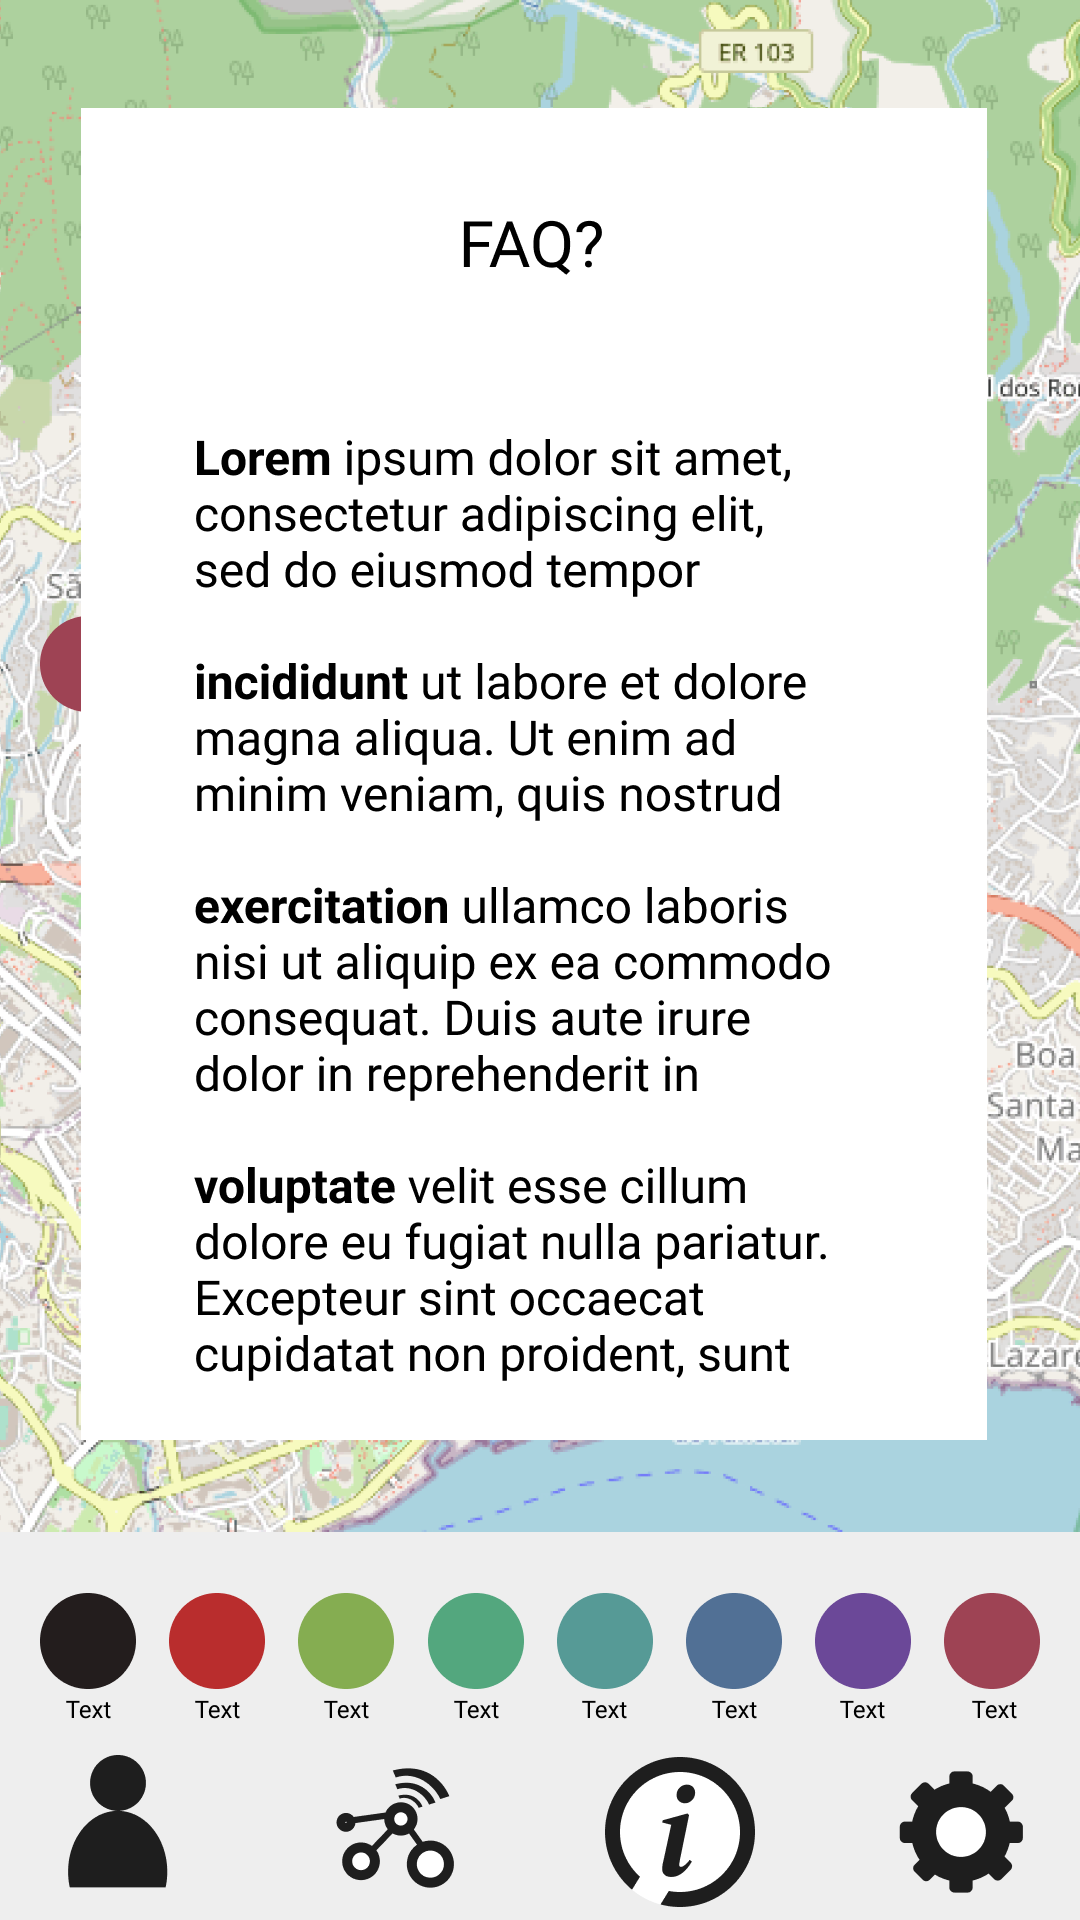
\includegraphics[width=130pt]{../assets/images/low_more_info.png}
        \caption{}
        \label{fig:lowfaq}
    \end{subfigure}%
    \caption{Low level prototype of (a) homepage, (b) about and (c) FAQ pages.}
    \label{fig:lowlevelprototype}
\end{figure}

After doing a rough prototype, some refinements were done to each page, like
adding colours and creating icons, which became eventually became a medium level
prototype. Figure \ref{fig:mediumlevelprototype} shows tree pages of the medium level
prototype, these being the homepage, about
and faq pages. This prototype has a navigation menu on the bottom where the
other pages of the application can be selected along with some information
above the page icons, this information is supposed to be the categories of
the devices, the logic would be that the user could tap one of these categories
and only devices of that category should be displayed on the map. It can
be seen that between the three pages the map stays in the background and
the various pages work like an overlay on the homepage, this would be
changed in subsequent prototype versions.

\begin{figure}
    \centering
    \begin{subfigure}{0.33\textwidth}
        \centering
        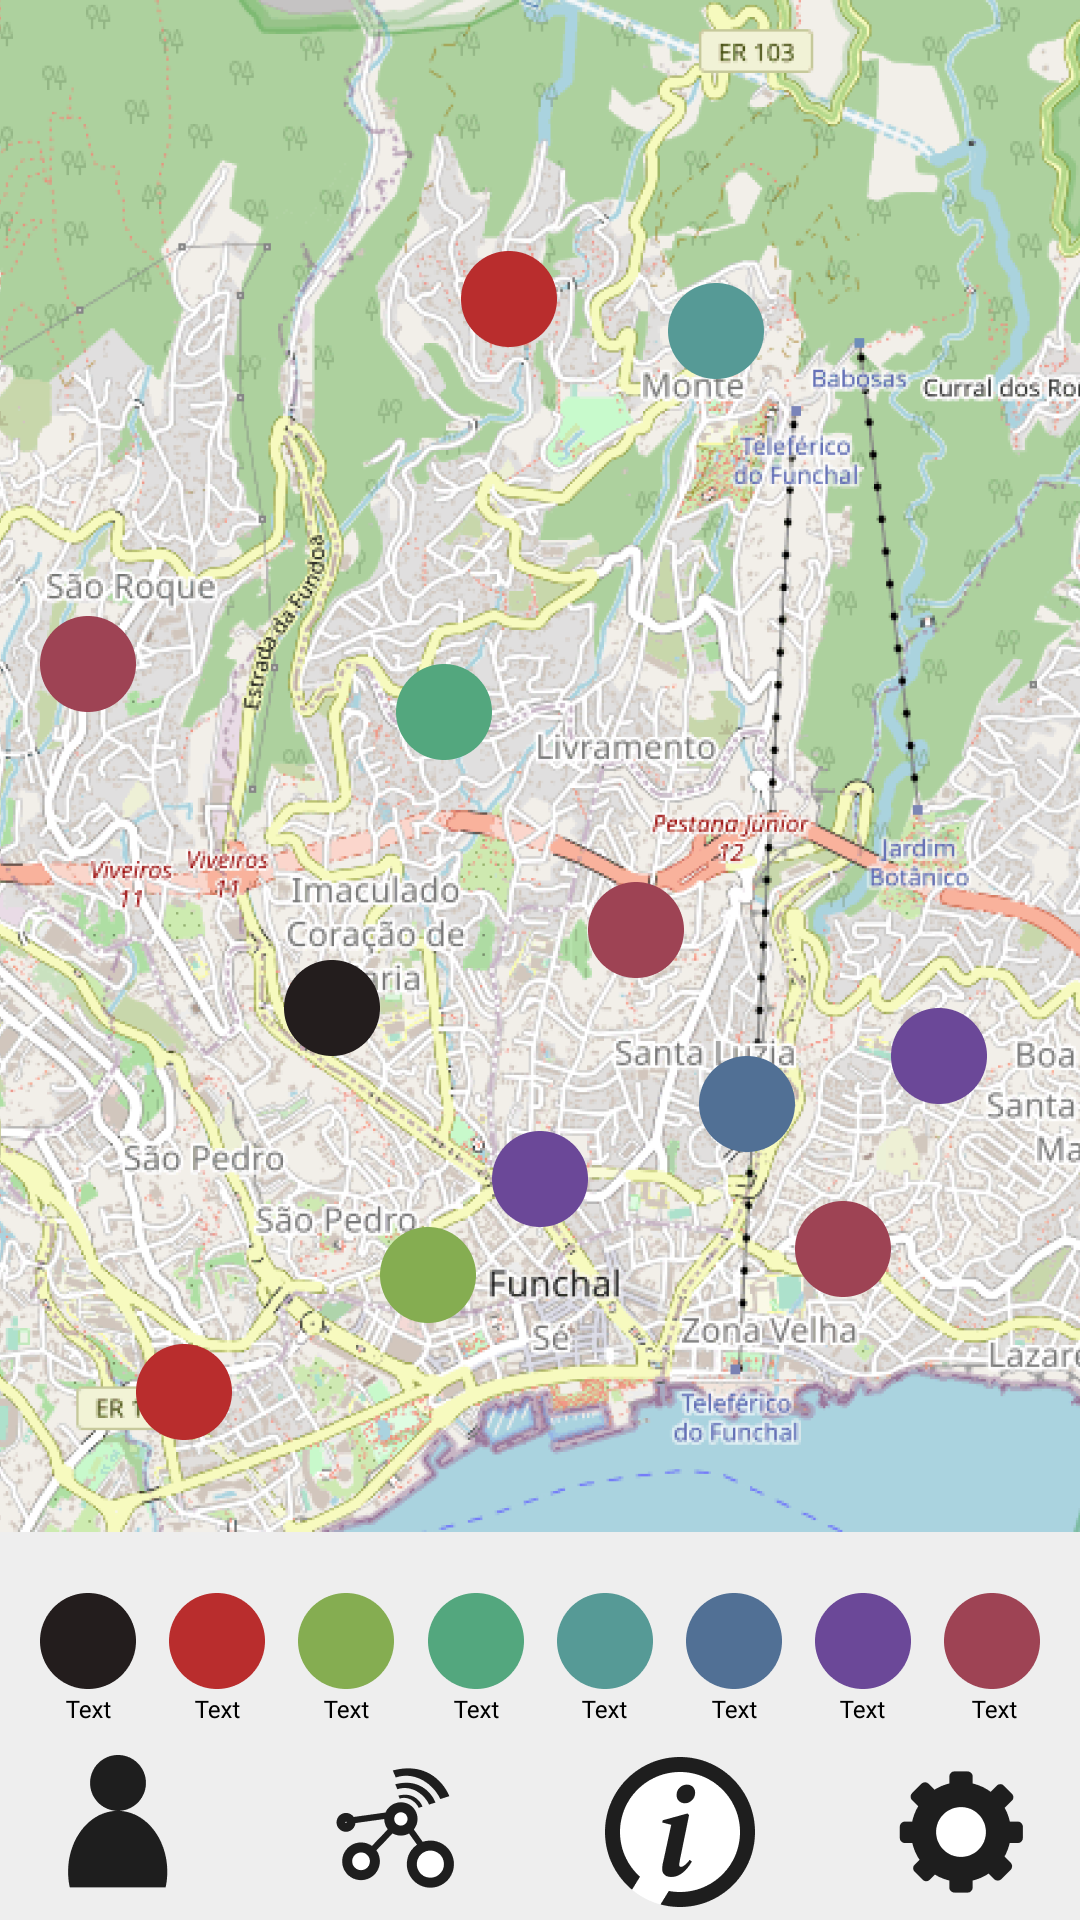
\includegraphics[width=130pt]{../assets/images/medium_homepage.png}
        \caption{}
        \label{fig:mediumhome}
    \end{subfigure}%
    \begin{subfigure}{0.33\textwidth}
        \centering
        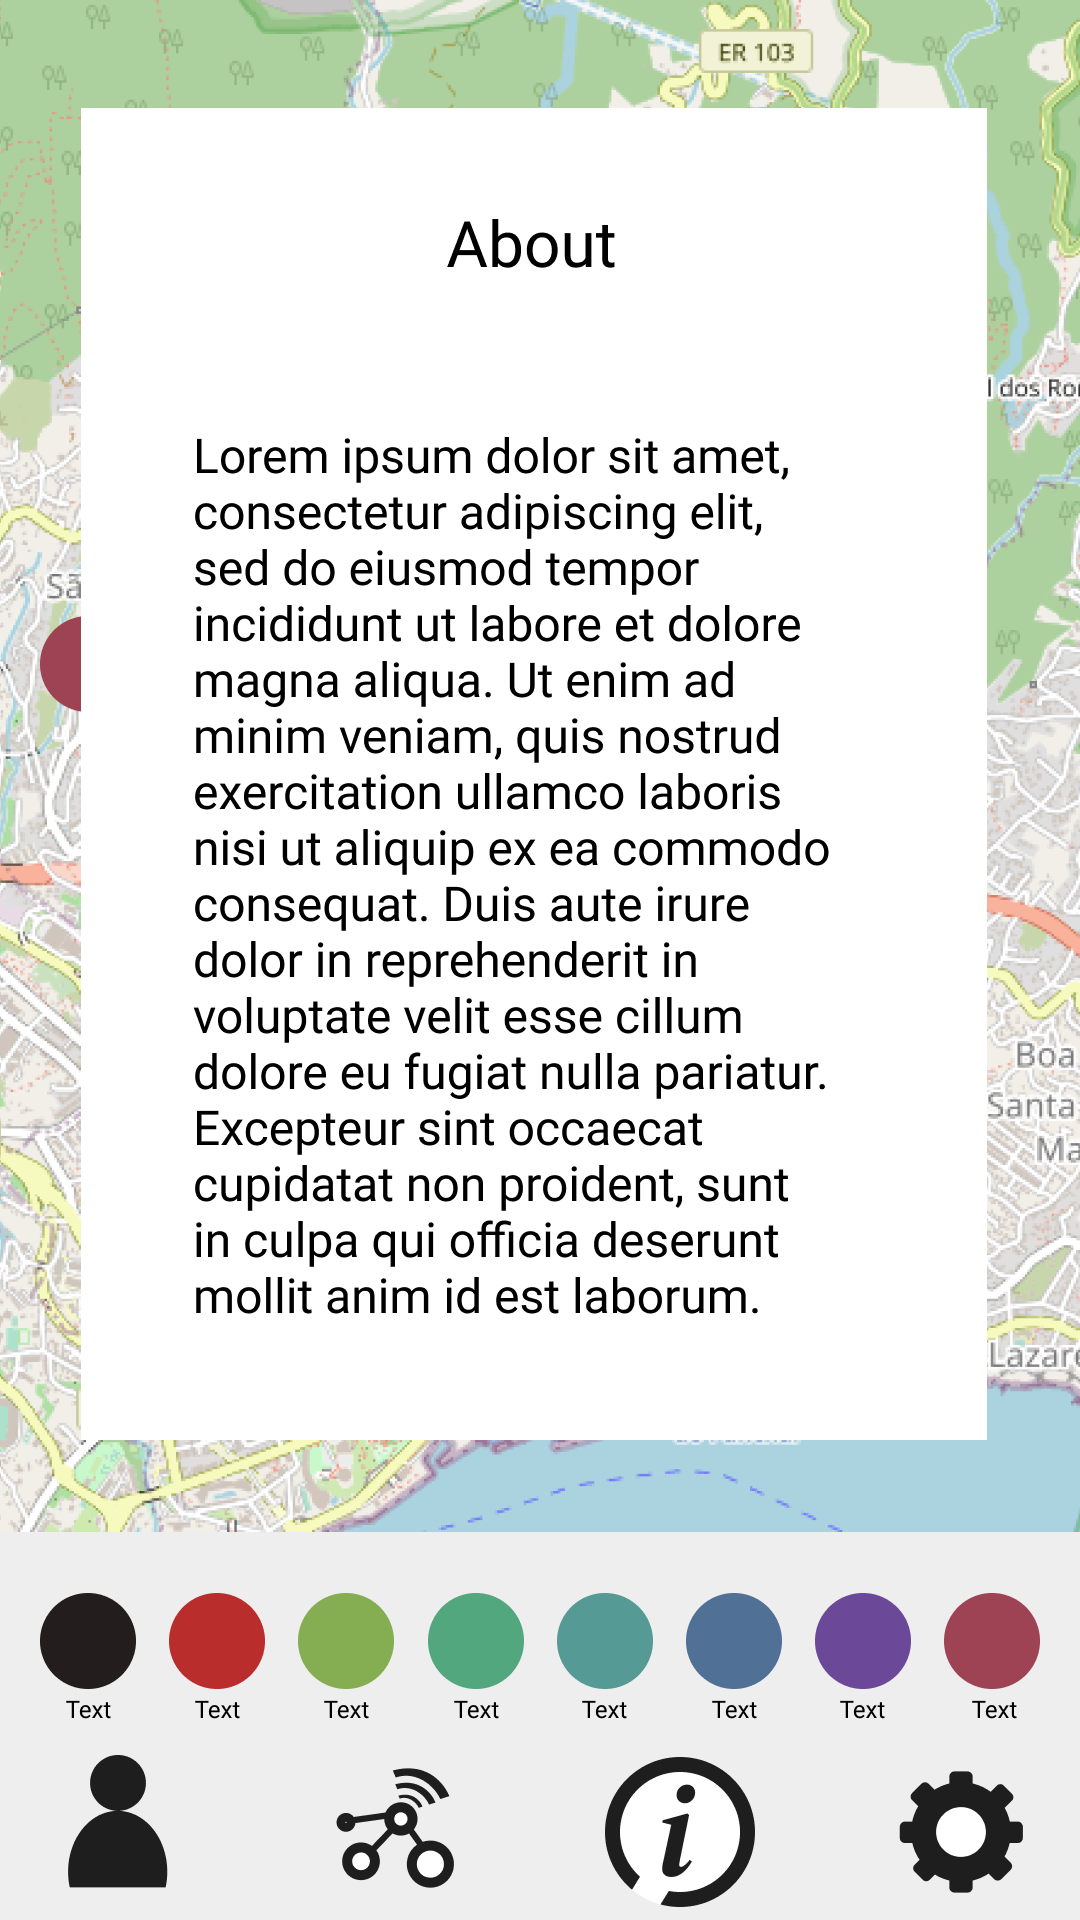
\includegraphics[width=130pt]{../assets/images/medium_about.png}
        \caption{}
        \label{fig:mediumabout}
    \end{subfigure}%
    \begin{subfigure}{0.33\textwidth}
        \centering
        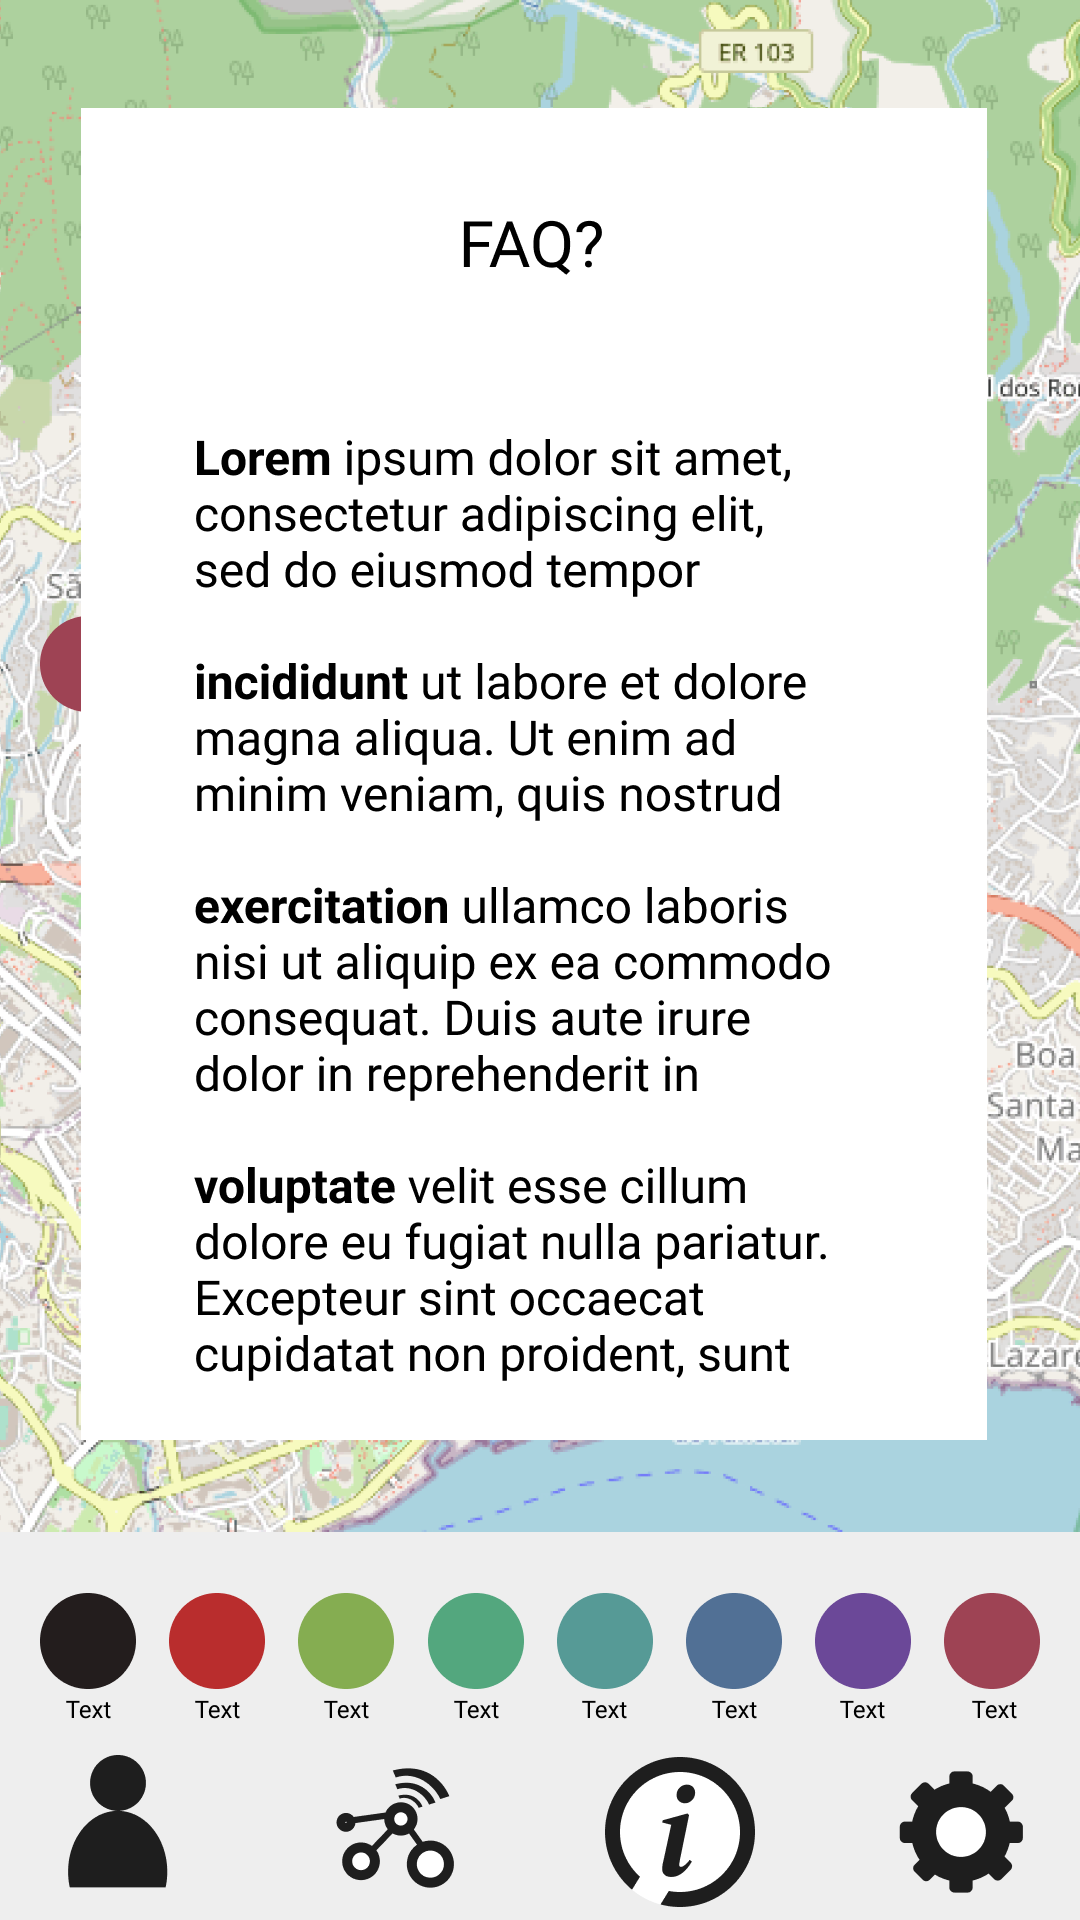
\includegraphics[width=130pt]{../assets/images/medium_more_info.png}
        \caption{}
        \label{fig:mediumfaq}
    \end{subfigure}%
    \caption{Medium level prototype of (a) homepage, (b) about and (c) FAQ pages.}
    \label{fig:mediumlevelprototype}
\end{figure}

Another prototype version was created, this being the final one before
the developed version. The high level version can be seen in Figure \ref{fig:highlevelprototype}
which shows three pages: homepage, FAQ and IoT devices. This is the version
that more closely resembles the developed application, although some design
elements were changed. Between the medium and high level prototypes, more icons
were created, colours were changed and other pages were designed. More icons
to the navigation footer were created, namely for the homepage and faq pages
which were missing from previous versions even with those pages being designed.
An icon for each category was also created, these show up on the map, representing
the type of device, and also on the devices page, so that devices can be quickly
identified.

\begin{figure}[H]
    \centering
    \begin{subfigure}{0.33\textwidth}
        \centering
        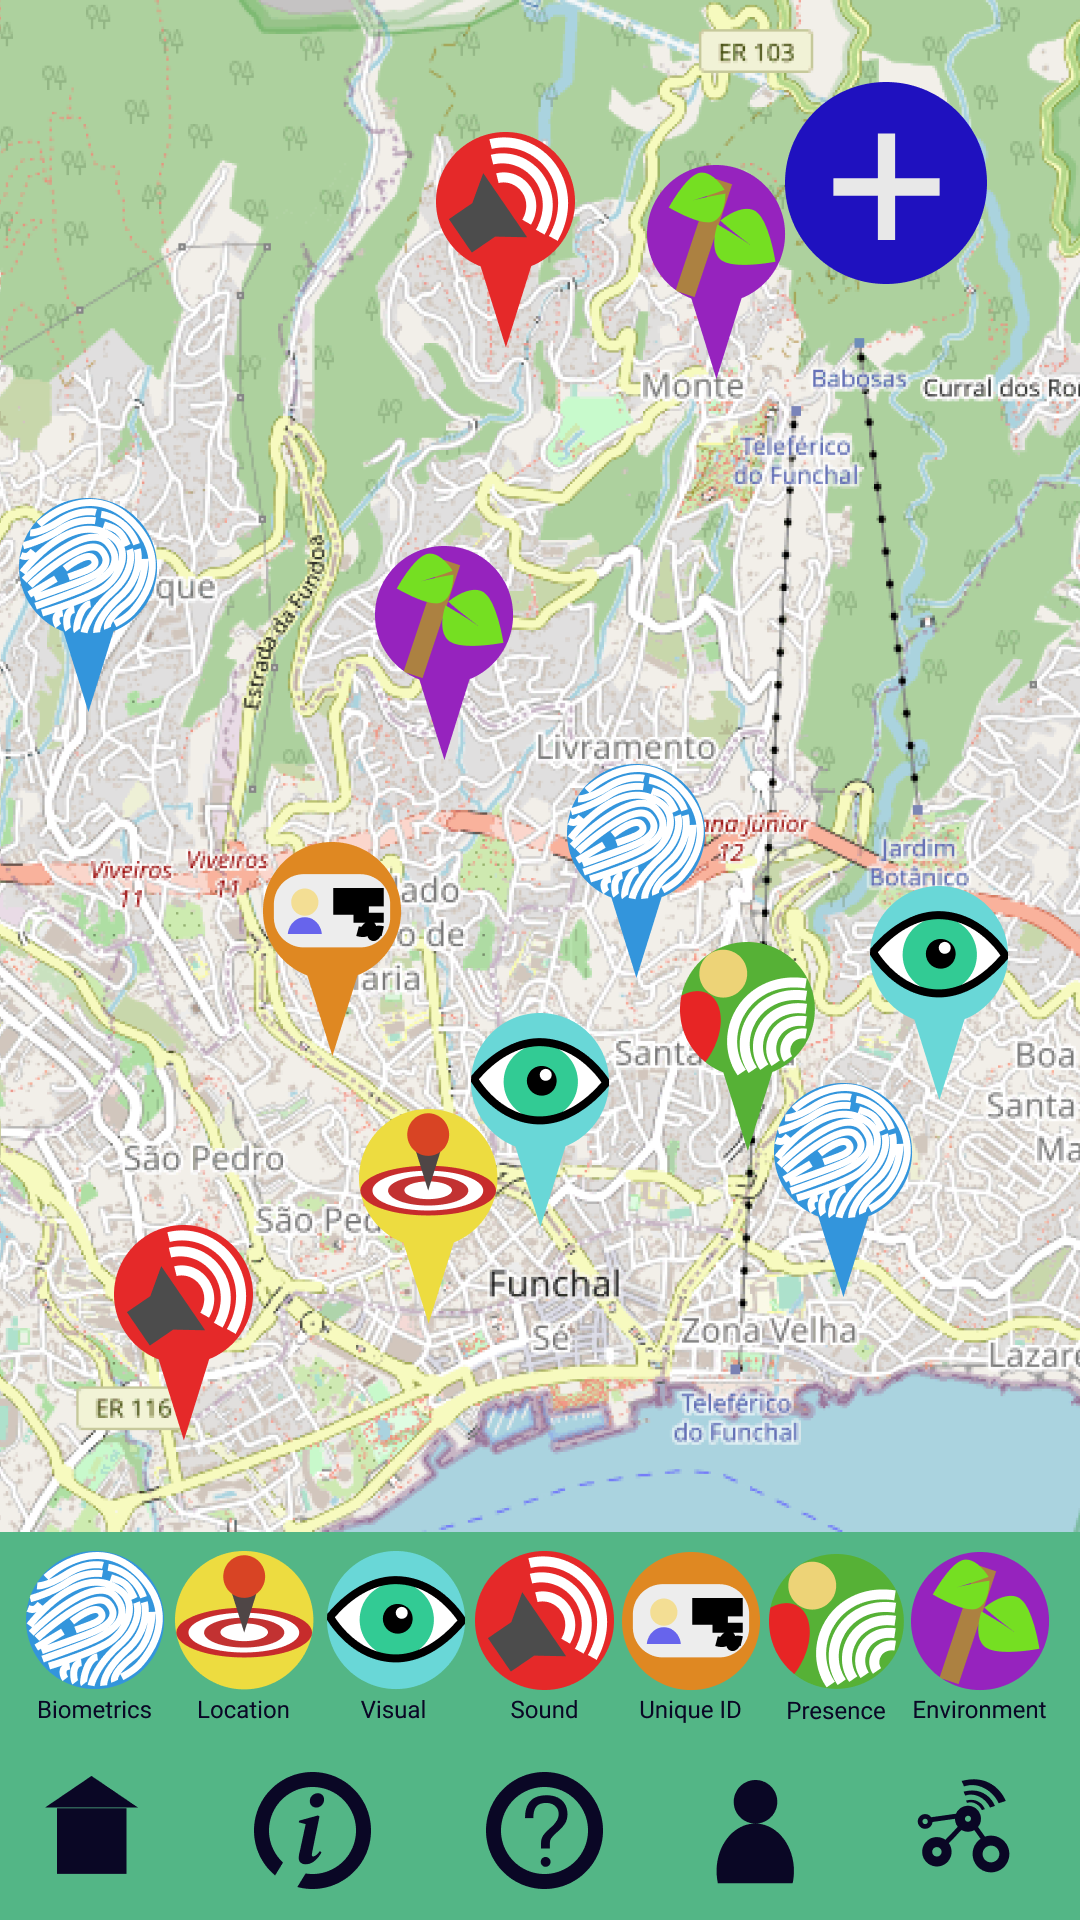
\includegraphics[width=130pt]{../assets/images/high_homepage.png}
        \caption{}
        \label{fig:highhome}
    \end{subfigure}%
    \begin{subfigure}{0.33\textwidth}
        \centering
        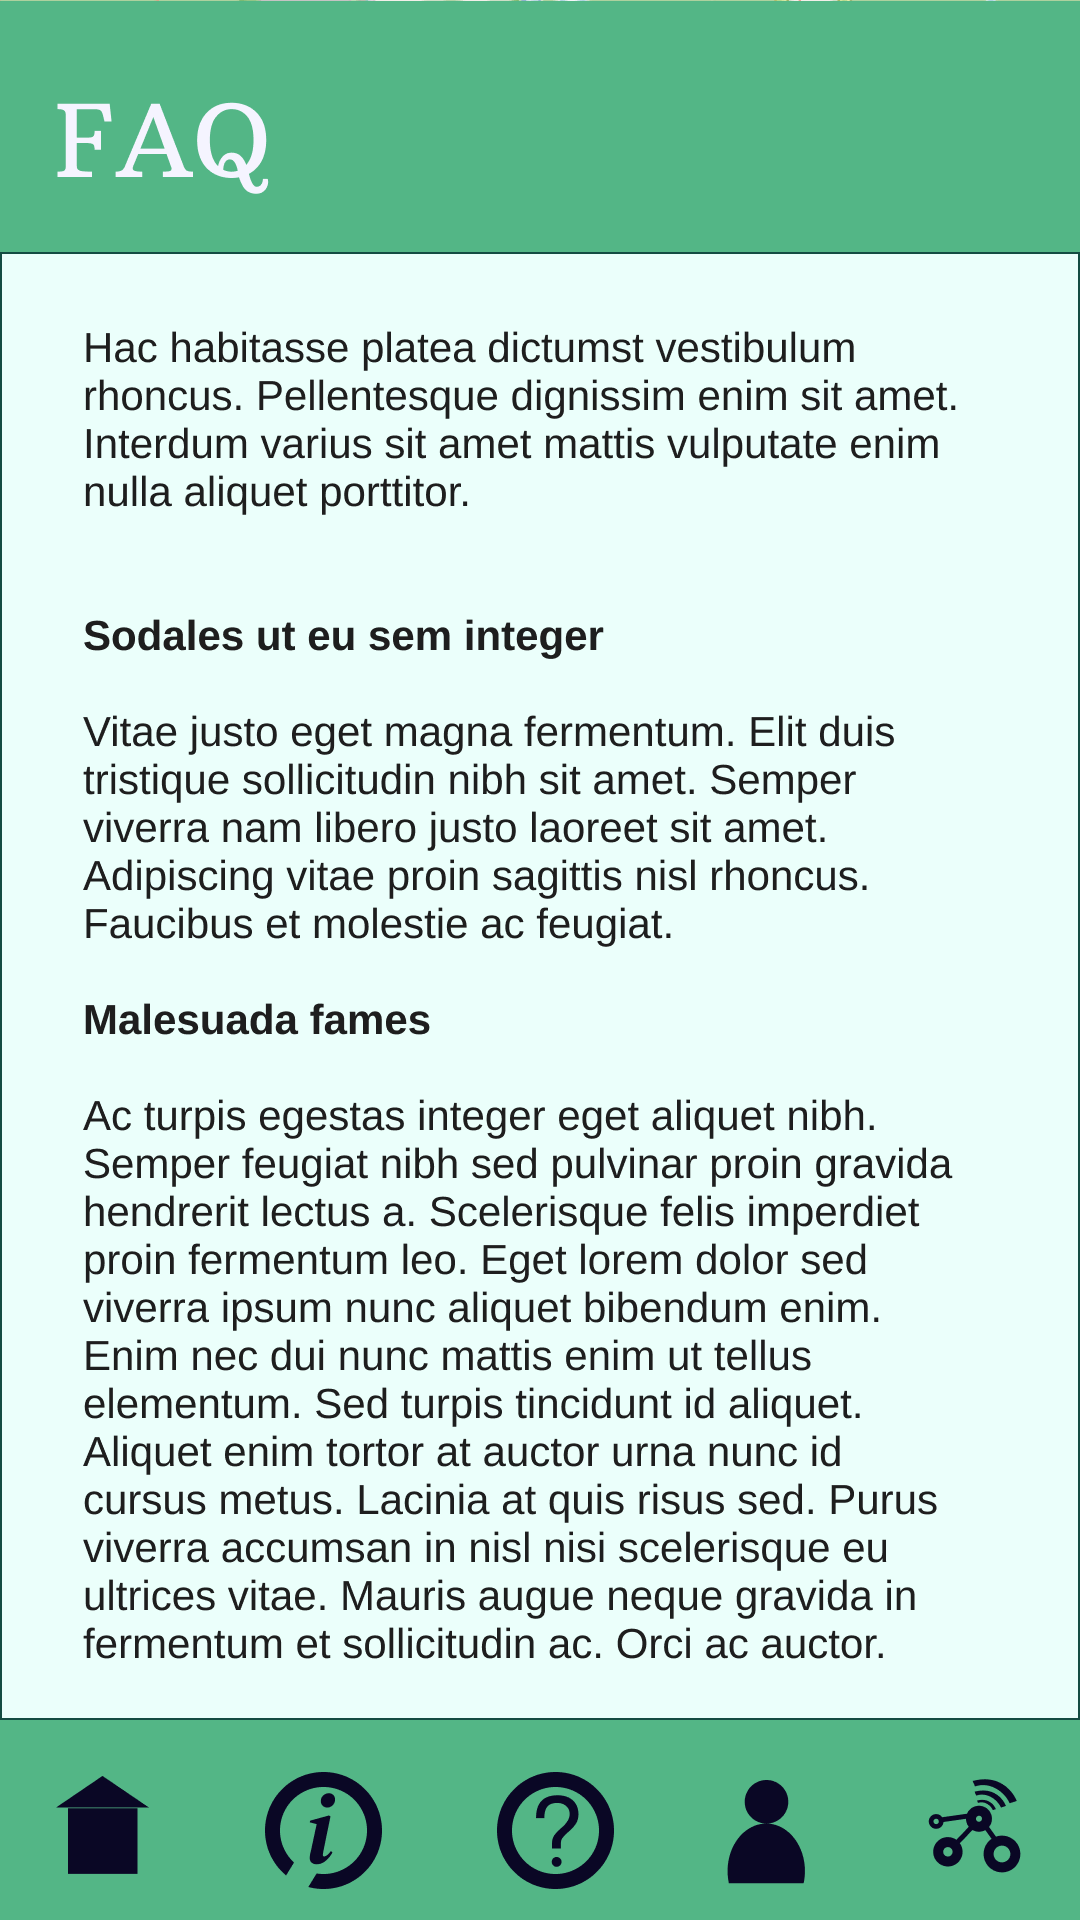
\includegraphics[width=130pt]{../assets/images/high_more_info.png}
        \caption{}
        \label{fig:highabout}
    \end{subfigure}%
    \begin{subfigure}{0.33\textwidth}
        \centering
        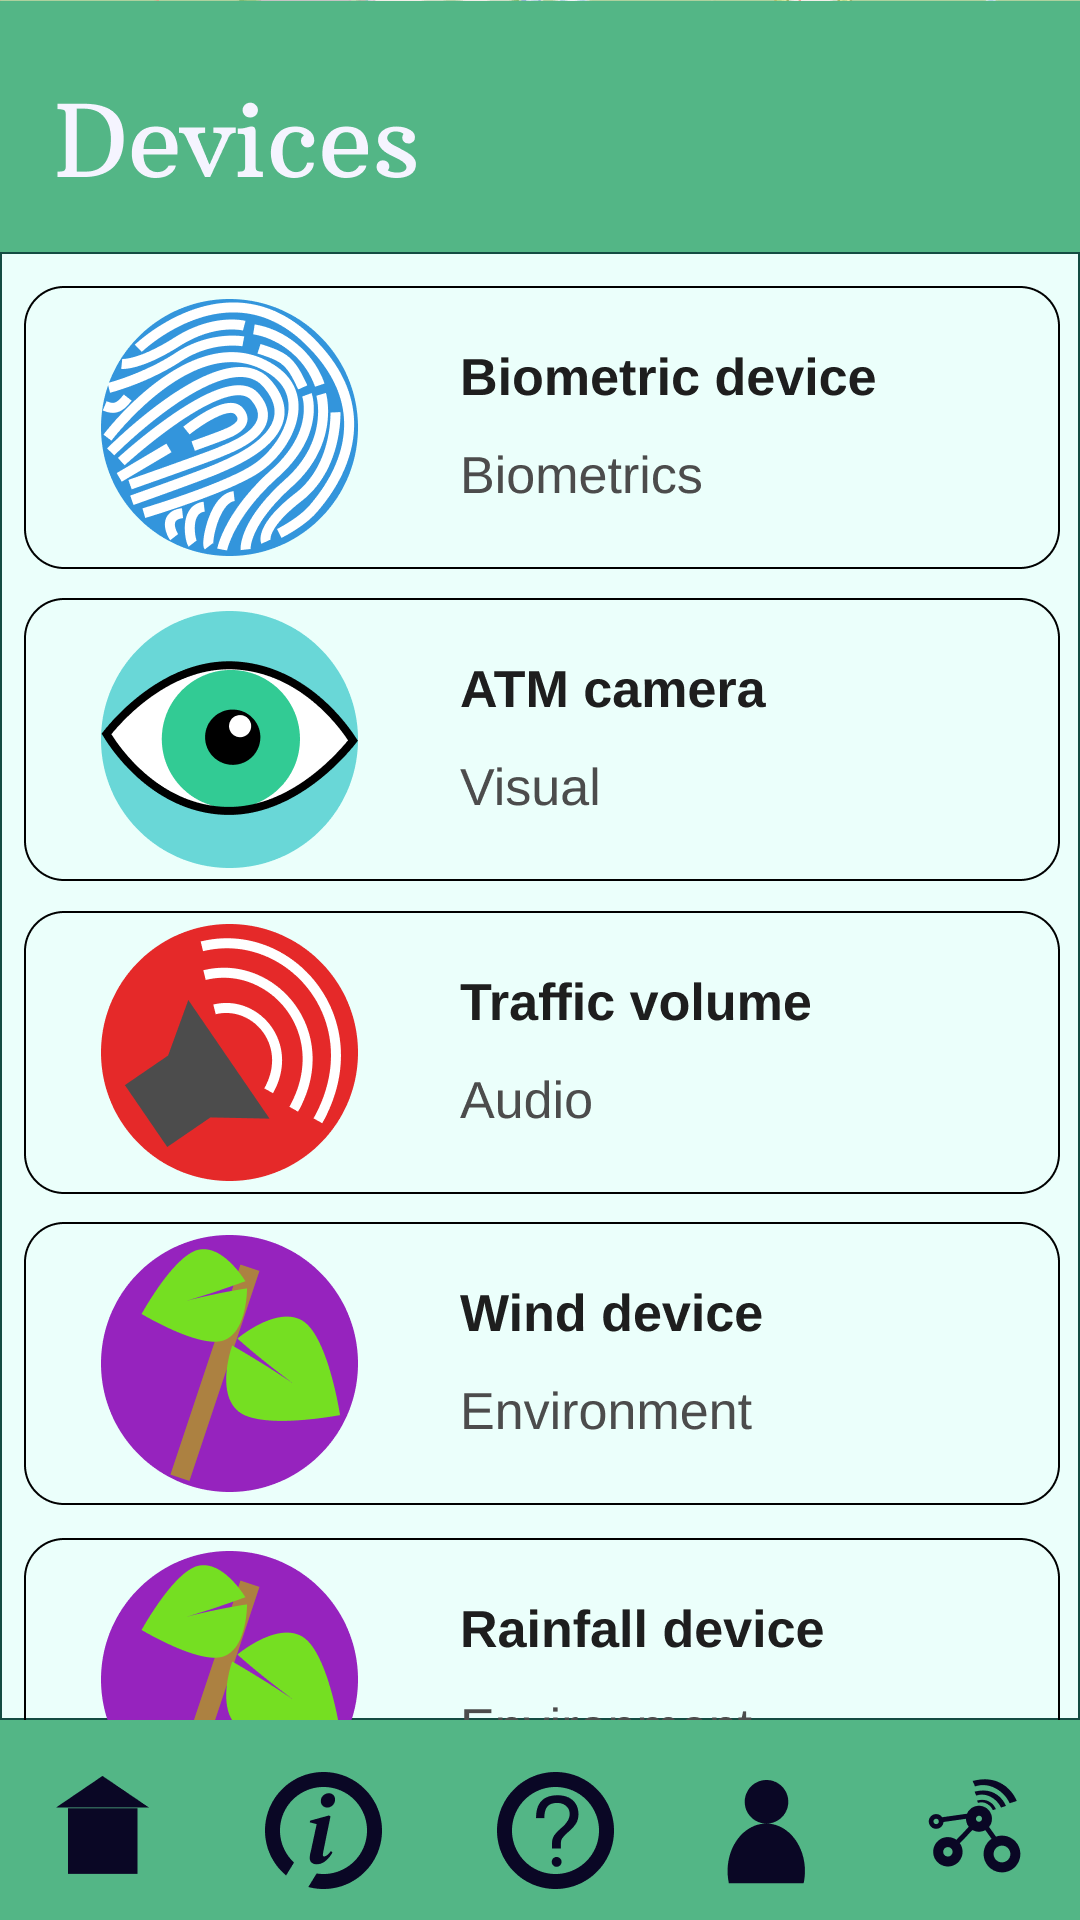
\includegraphics[width=130pt]{../assets/images/high_devices.png}
        \caption{}
        \label{fig:highfaq}
    \end{subfigure}%
    \caption{High level prototype of (a) homepage, (b) about and (c) FAQ pages.}
    \label{fig:highlevelprototype}
\end{figure}

After doing the prototypes, development was started, although some overlap
happened with the high level version prototype, as the icons for the categories
were being created. Figure \ref{fig:live_app} represents the application pages:
(\ref{fig:livehome}) homepage, (\ref{fig:liveabout}) about, (\ref{fig:livefaq}) more
information, (\ref{fig:live_devices}) IoT devices, (\ref{fig:live_device_info}) device
and (\ref{fig:live_statistics}) statistics.
Further changes would occur between the prototypes and
the application, such as the colour scheme, icons for pages that were created
were not used.

\begin{figure}[H]
    \centering
    \begin{subfigure}{0.30\textwidth}
        \centering
        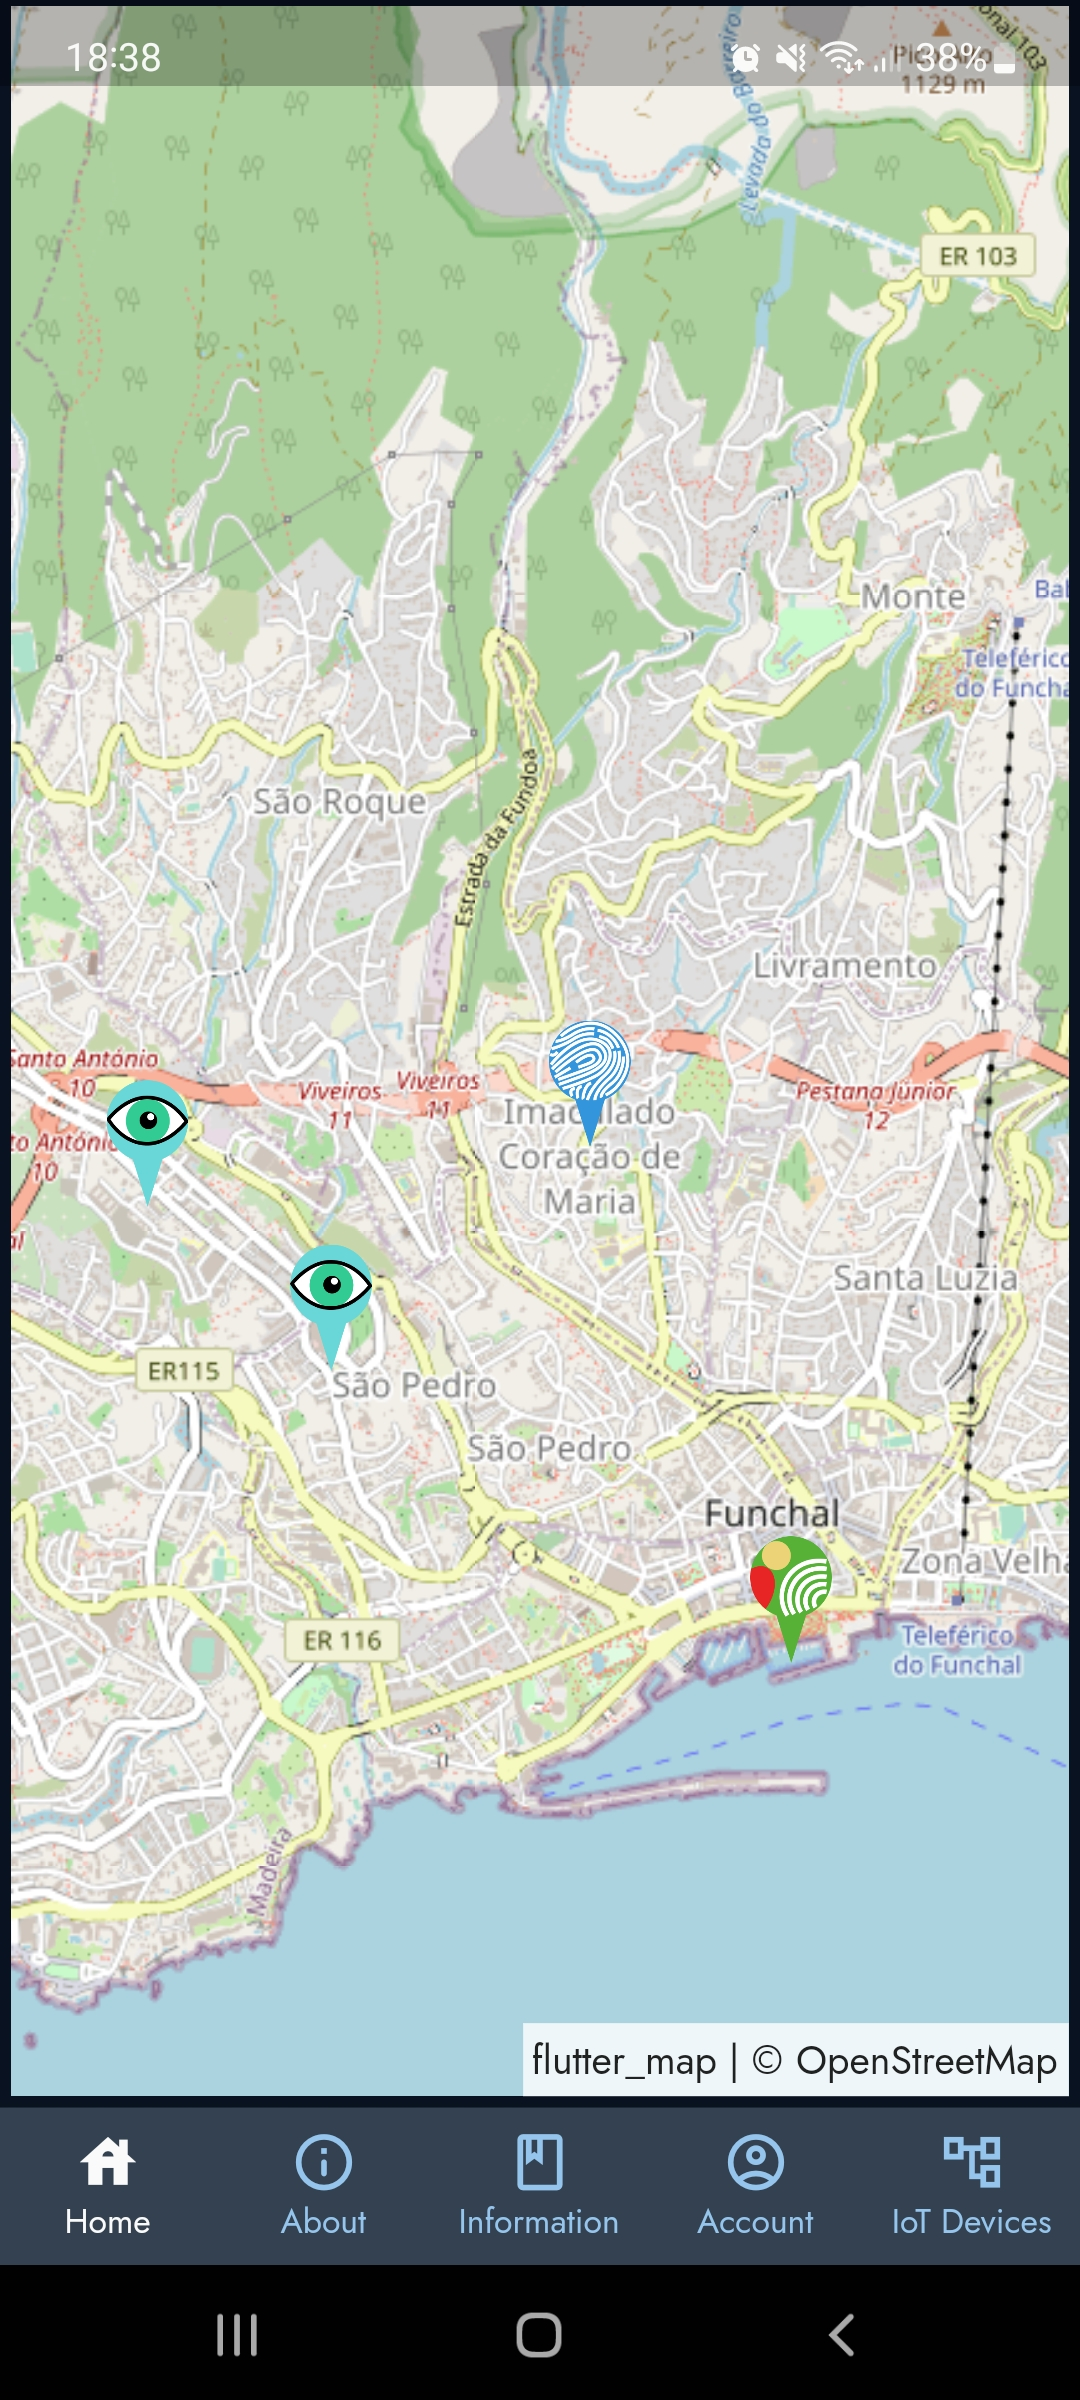
\includegraphics[width=125pt]{../assets/images/live_homepage.jpg}
        \caption{}
        \label{fig:livehome}
    \end{subfigure}
    \begin{subfigure}{0.30\textwidth}
        \centering
        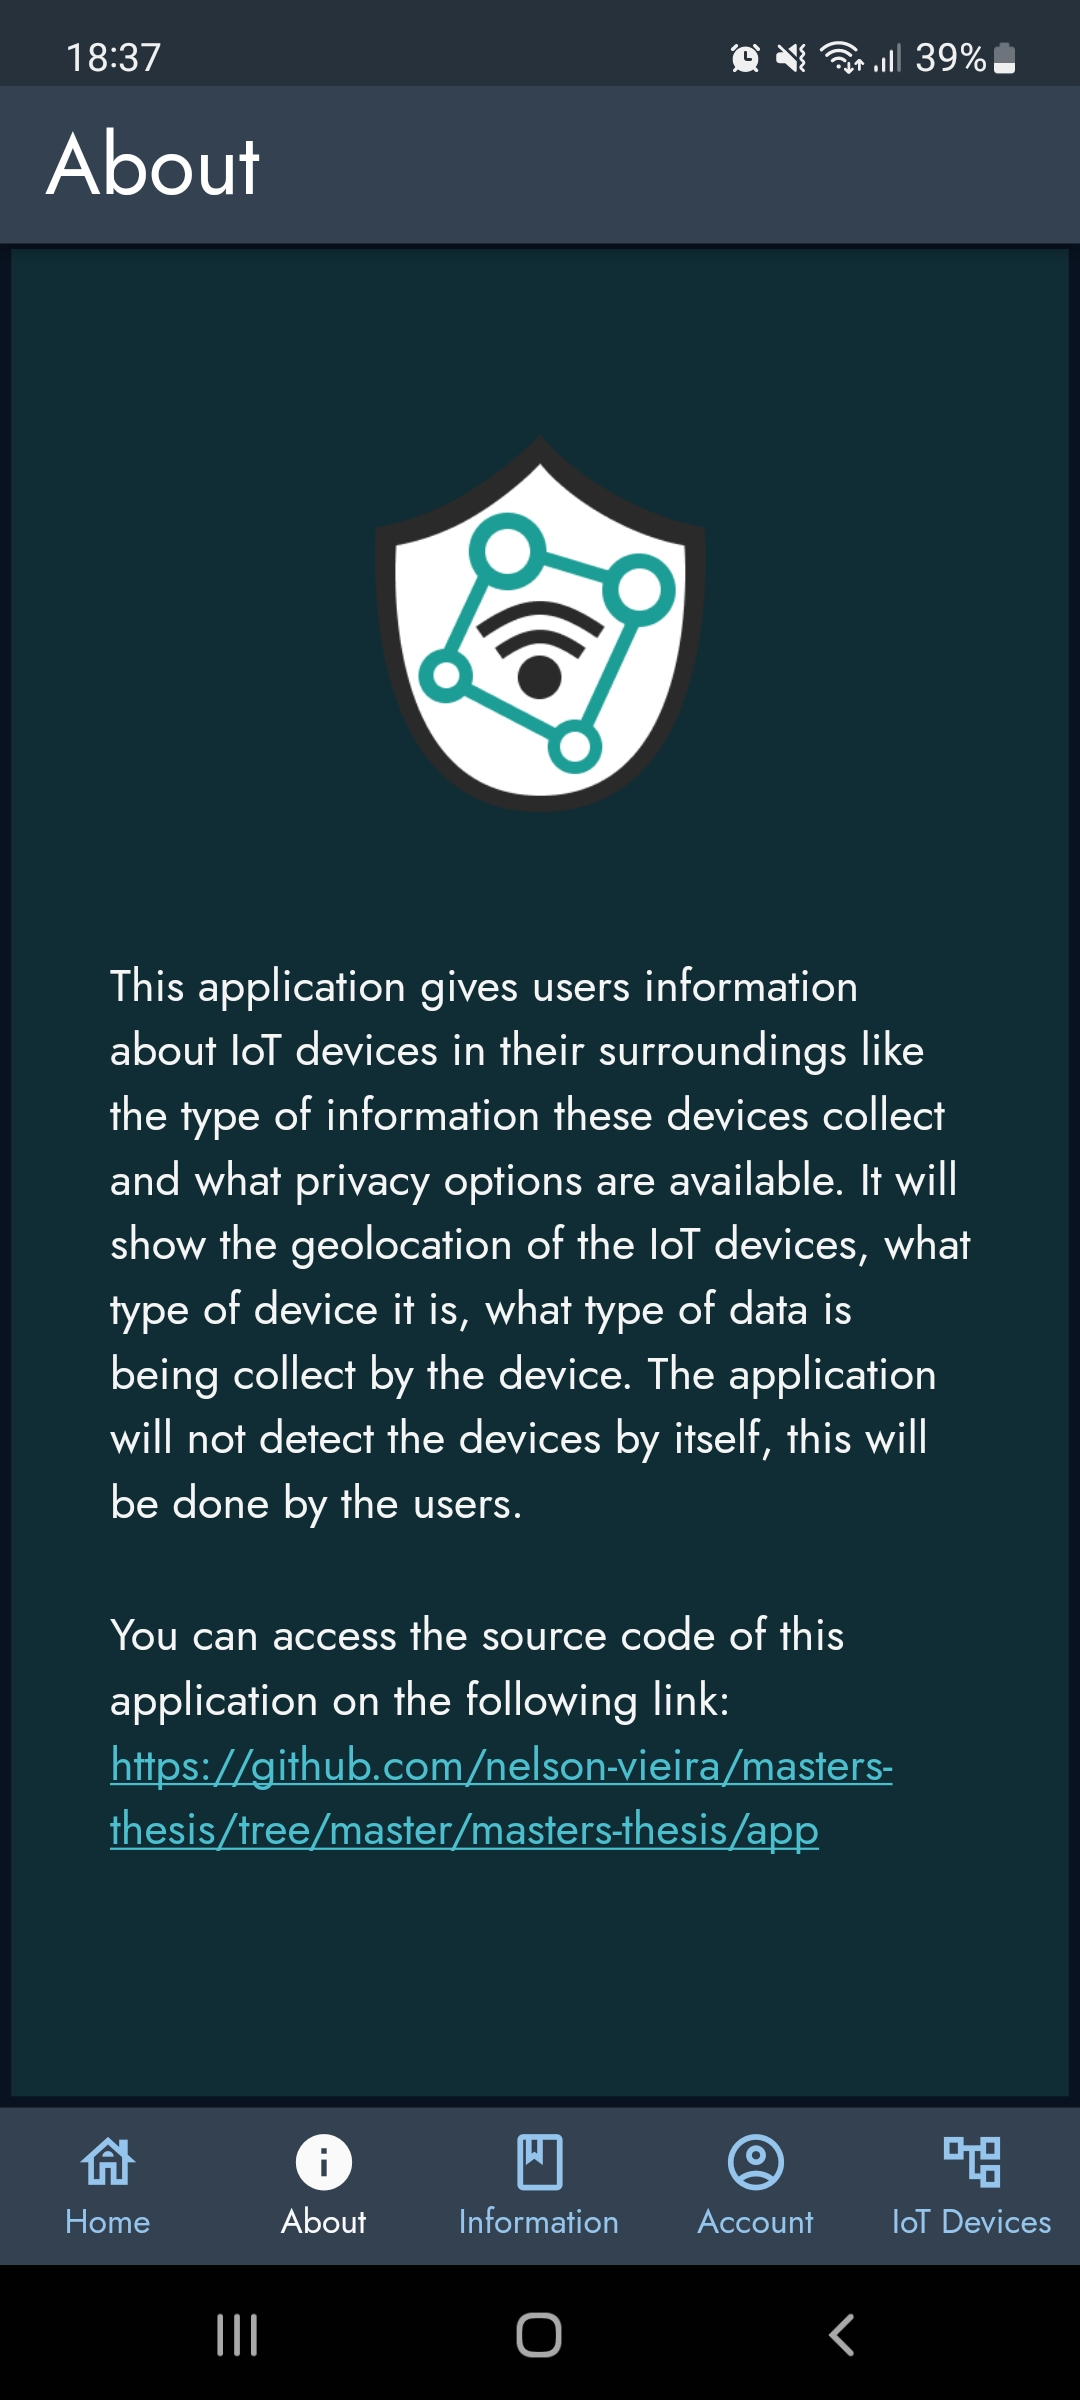
\includegraphics[width=125pt]{../assets/images/live_about.jpg}
        \caption{}
        \label{fig:liveabout}
    \end{subfigure}
    \begin{subfigure}{0.30\textwidth}
        \centering
        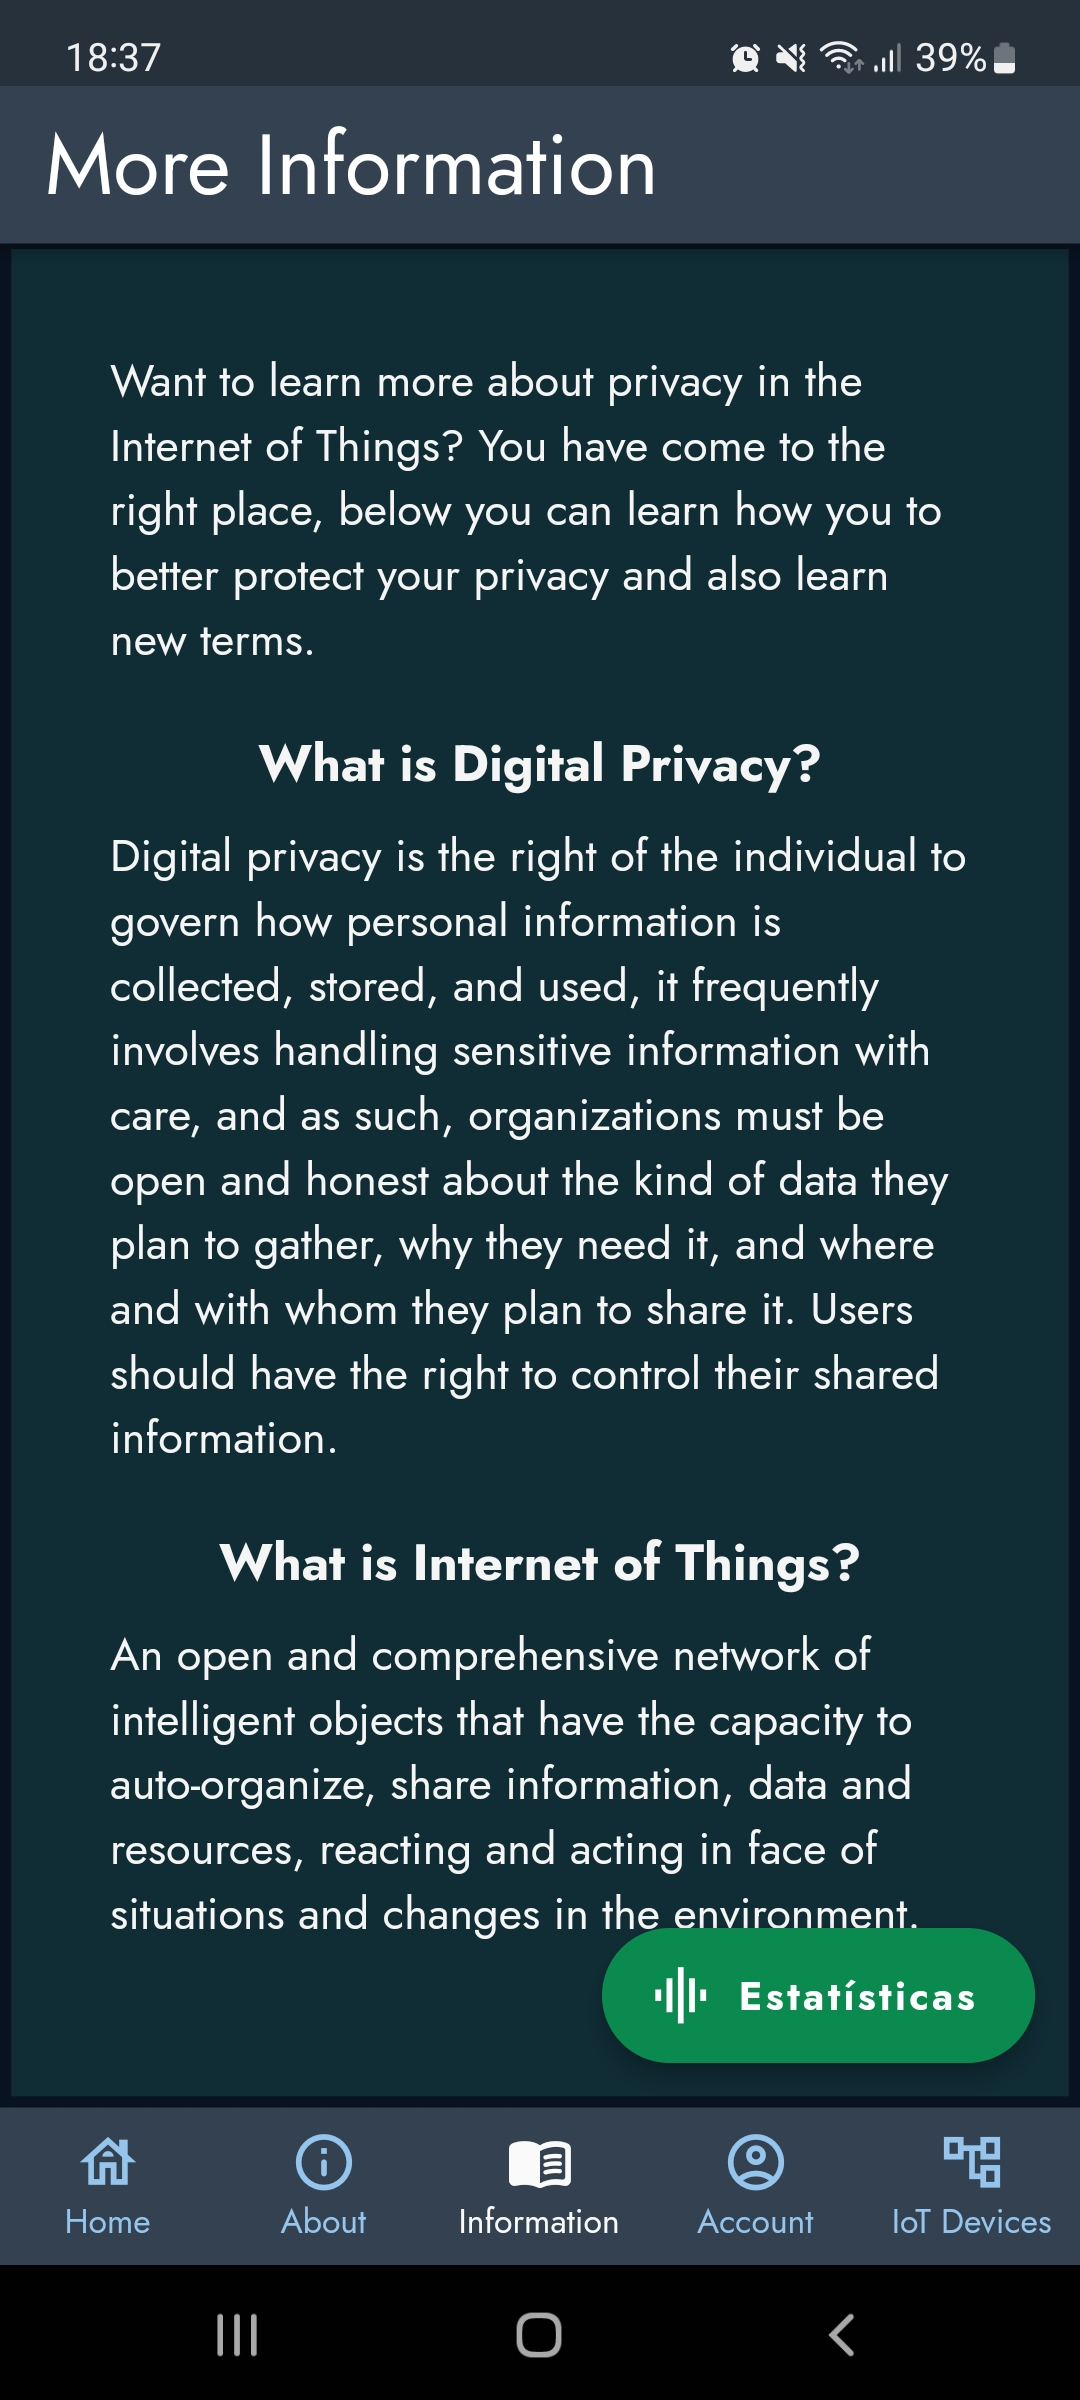
\includegraphics[width=125pt]{../assets/images/live_more_info.jpg}
        \caption{}
        \label{fig:livefaq}
    \end{subfigure}
    \begin{subfigure}{0.30\textwidth}
        \centering
        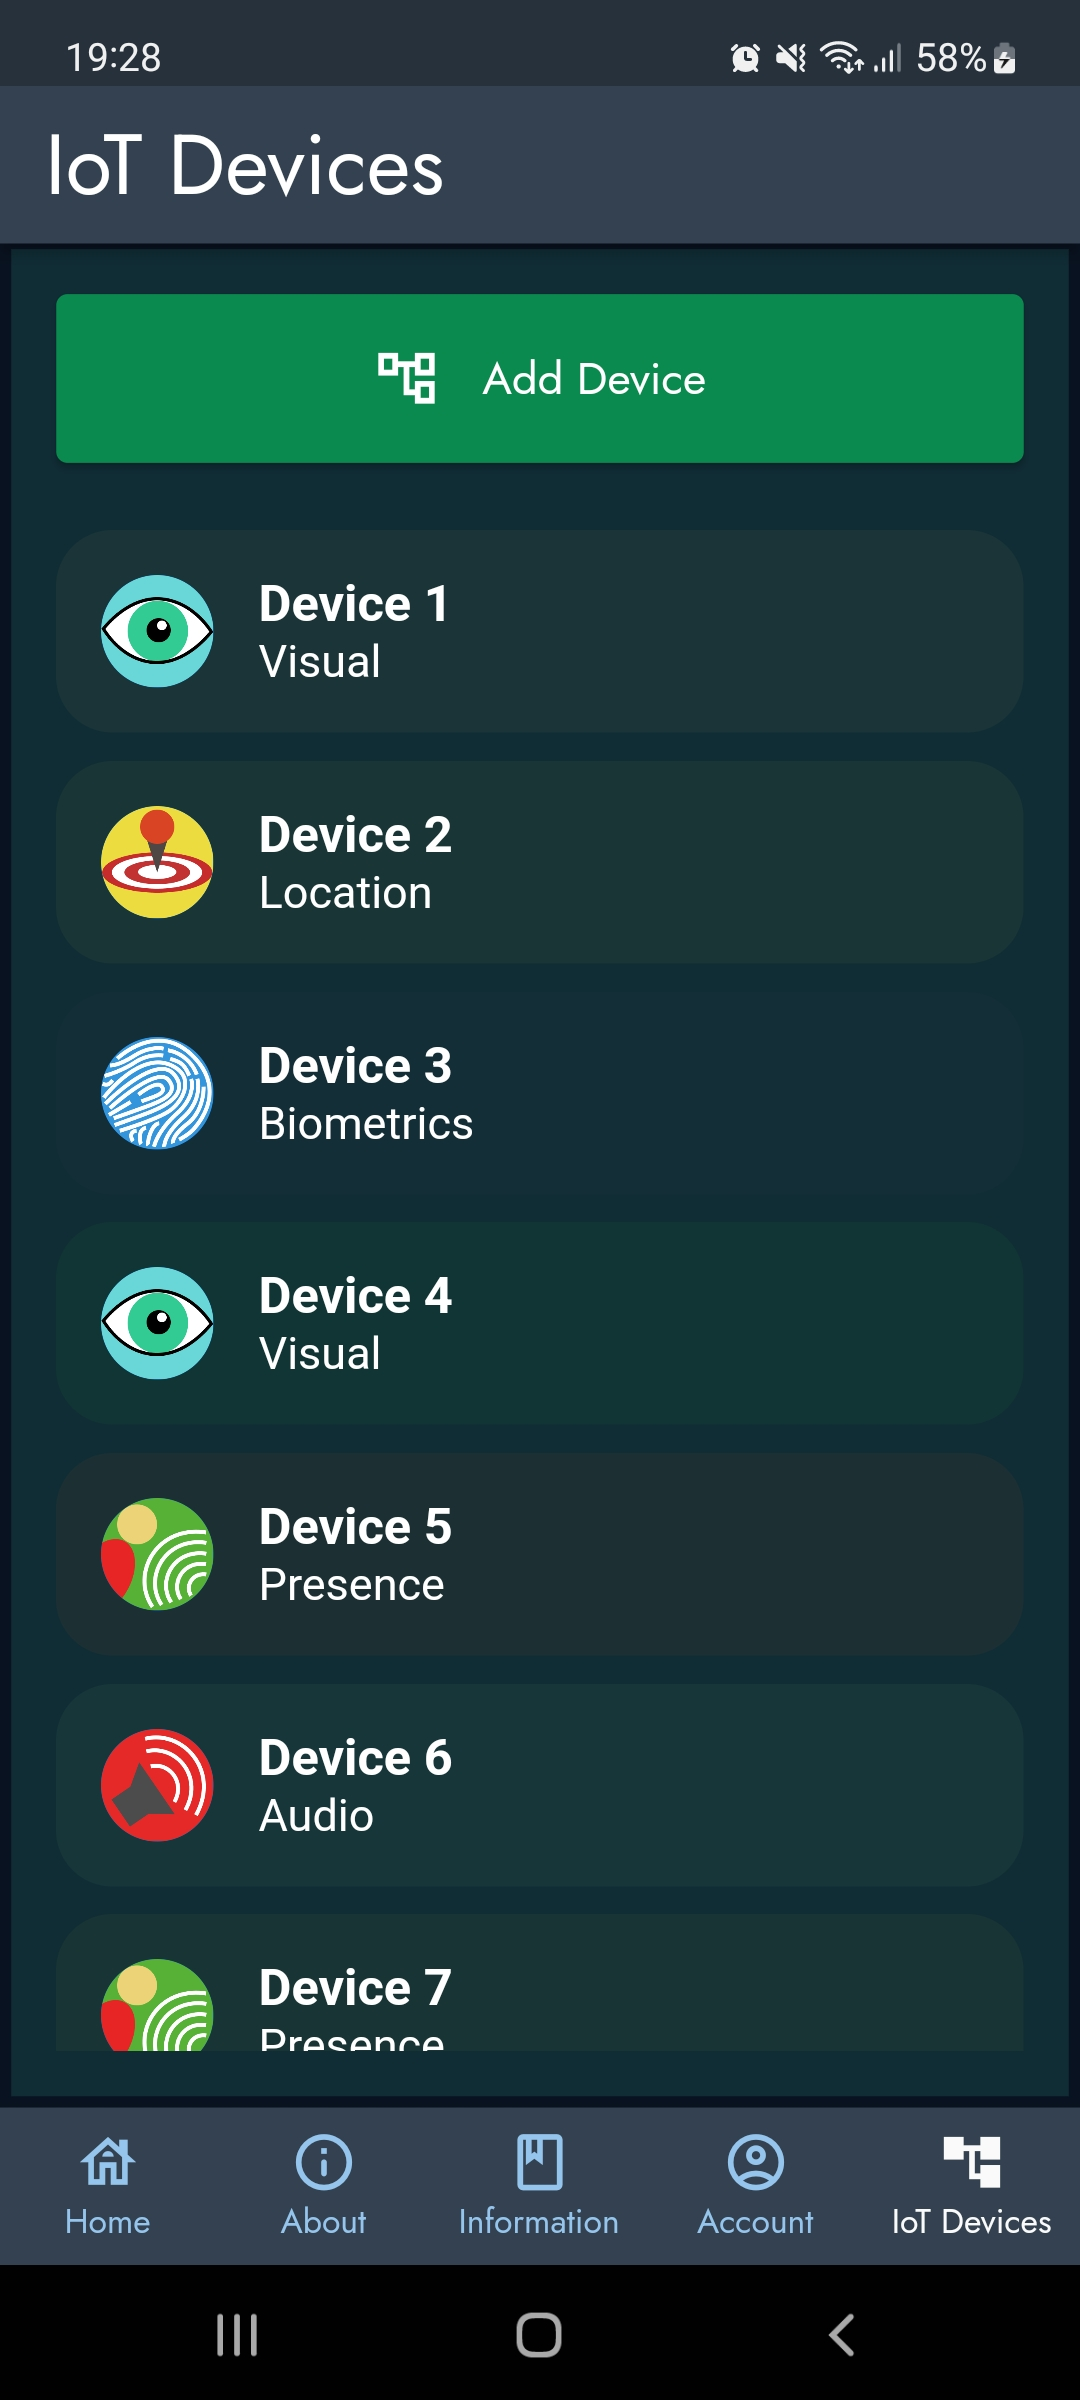
\includegraphics[width=125pt]{../assets/images/live_devices.jpg}
        \caption{}
        \label{fig:live_devices}
    \end{subfigure}
    \begin{subfigure}{0.30\textwidth}
        \centering
        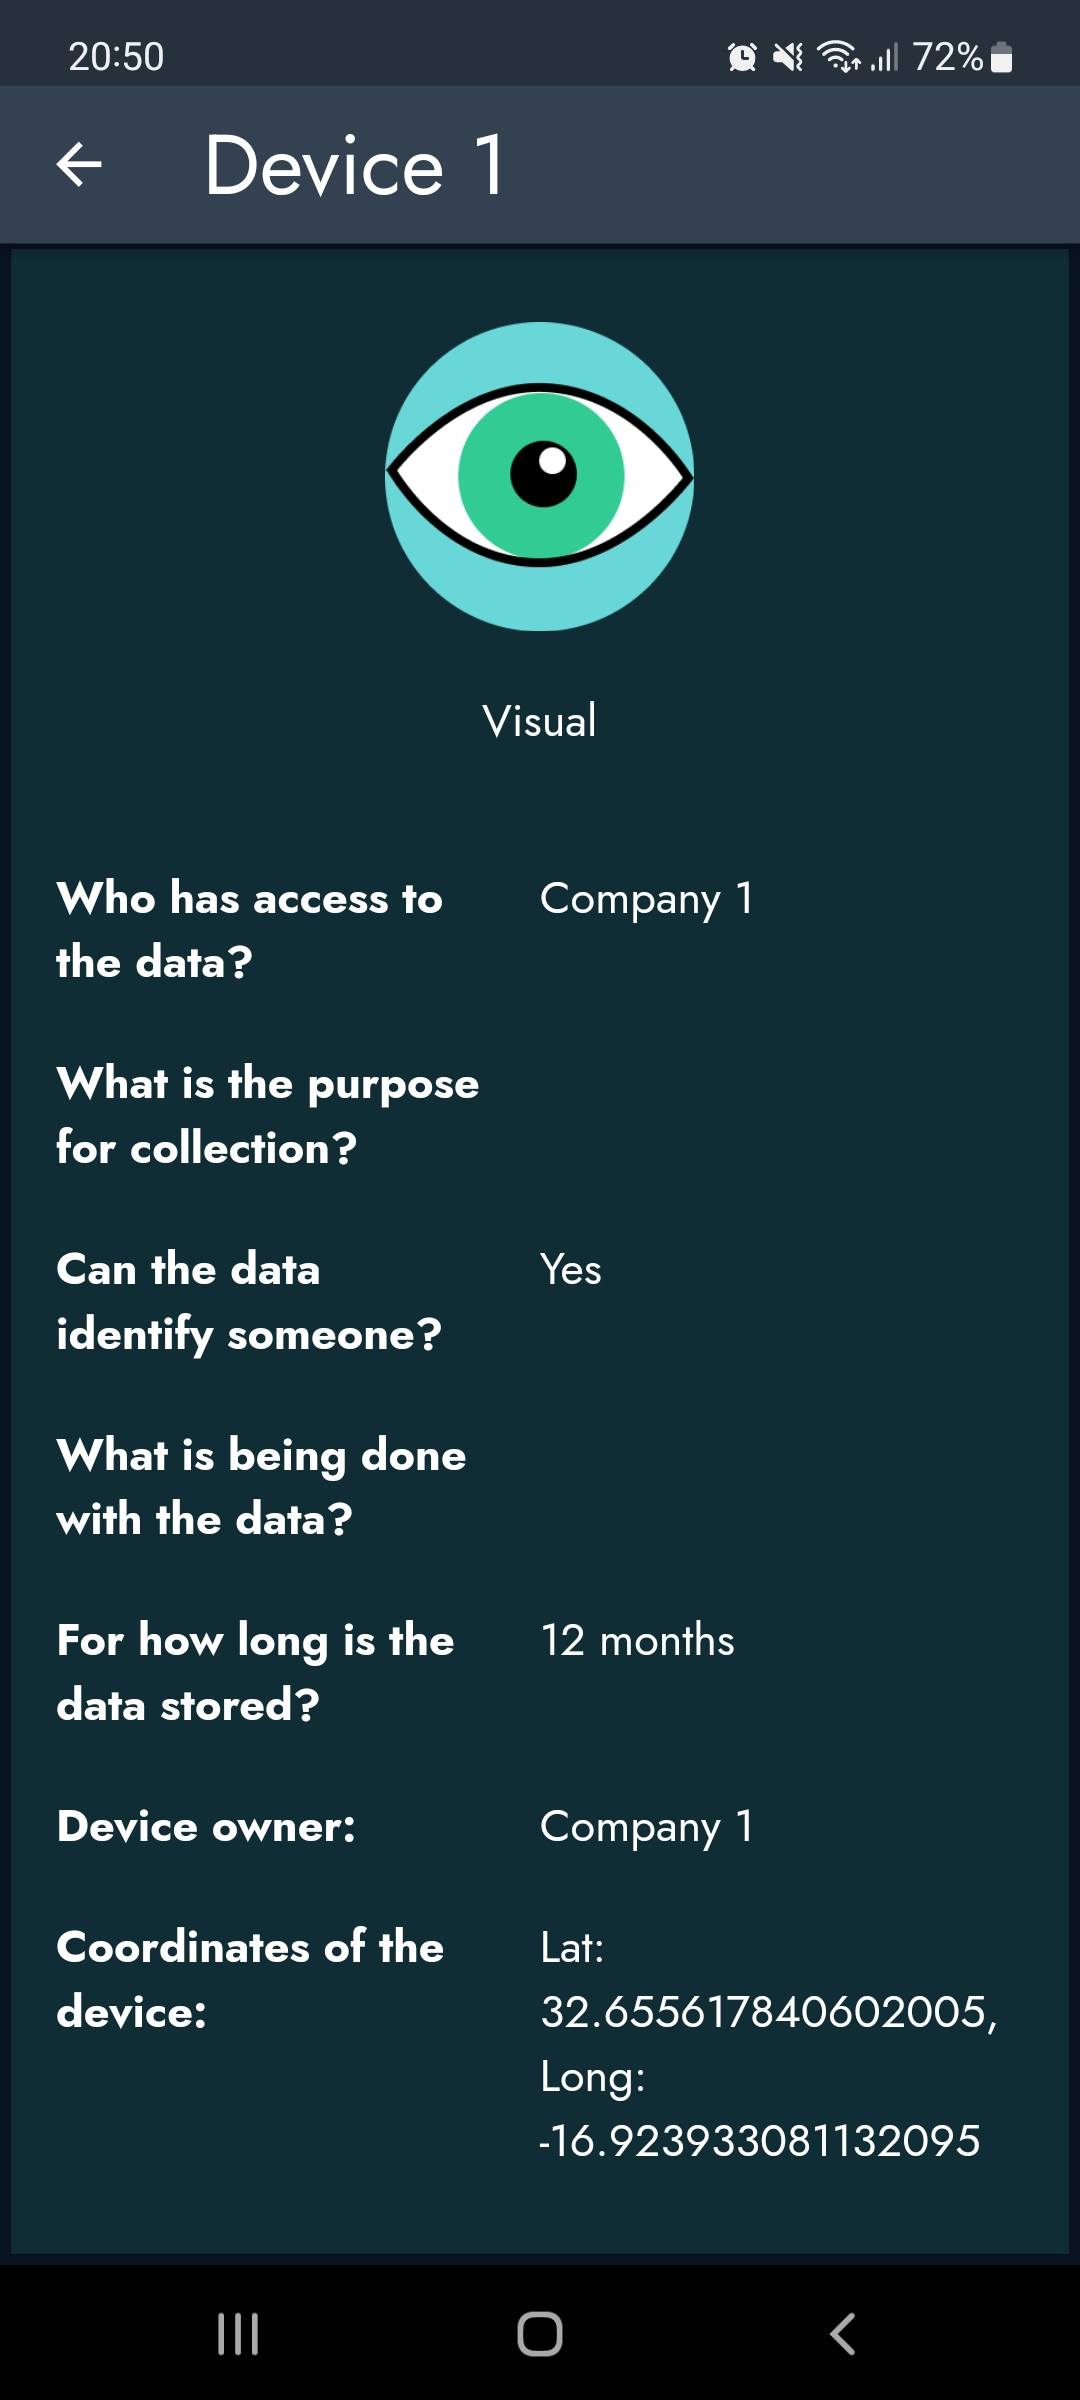
\includegraphics[width=125pt]{../assets/images/live_device_info.jpg}
        \caption{}
        \label{fig:live_device_info}
    \end{subfigure}
    \begin{subfigure}{0.30\textwidth}
        \centering
        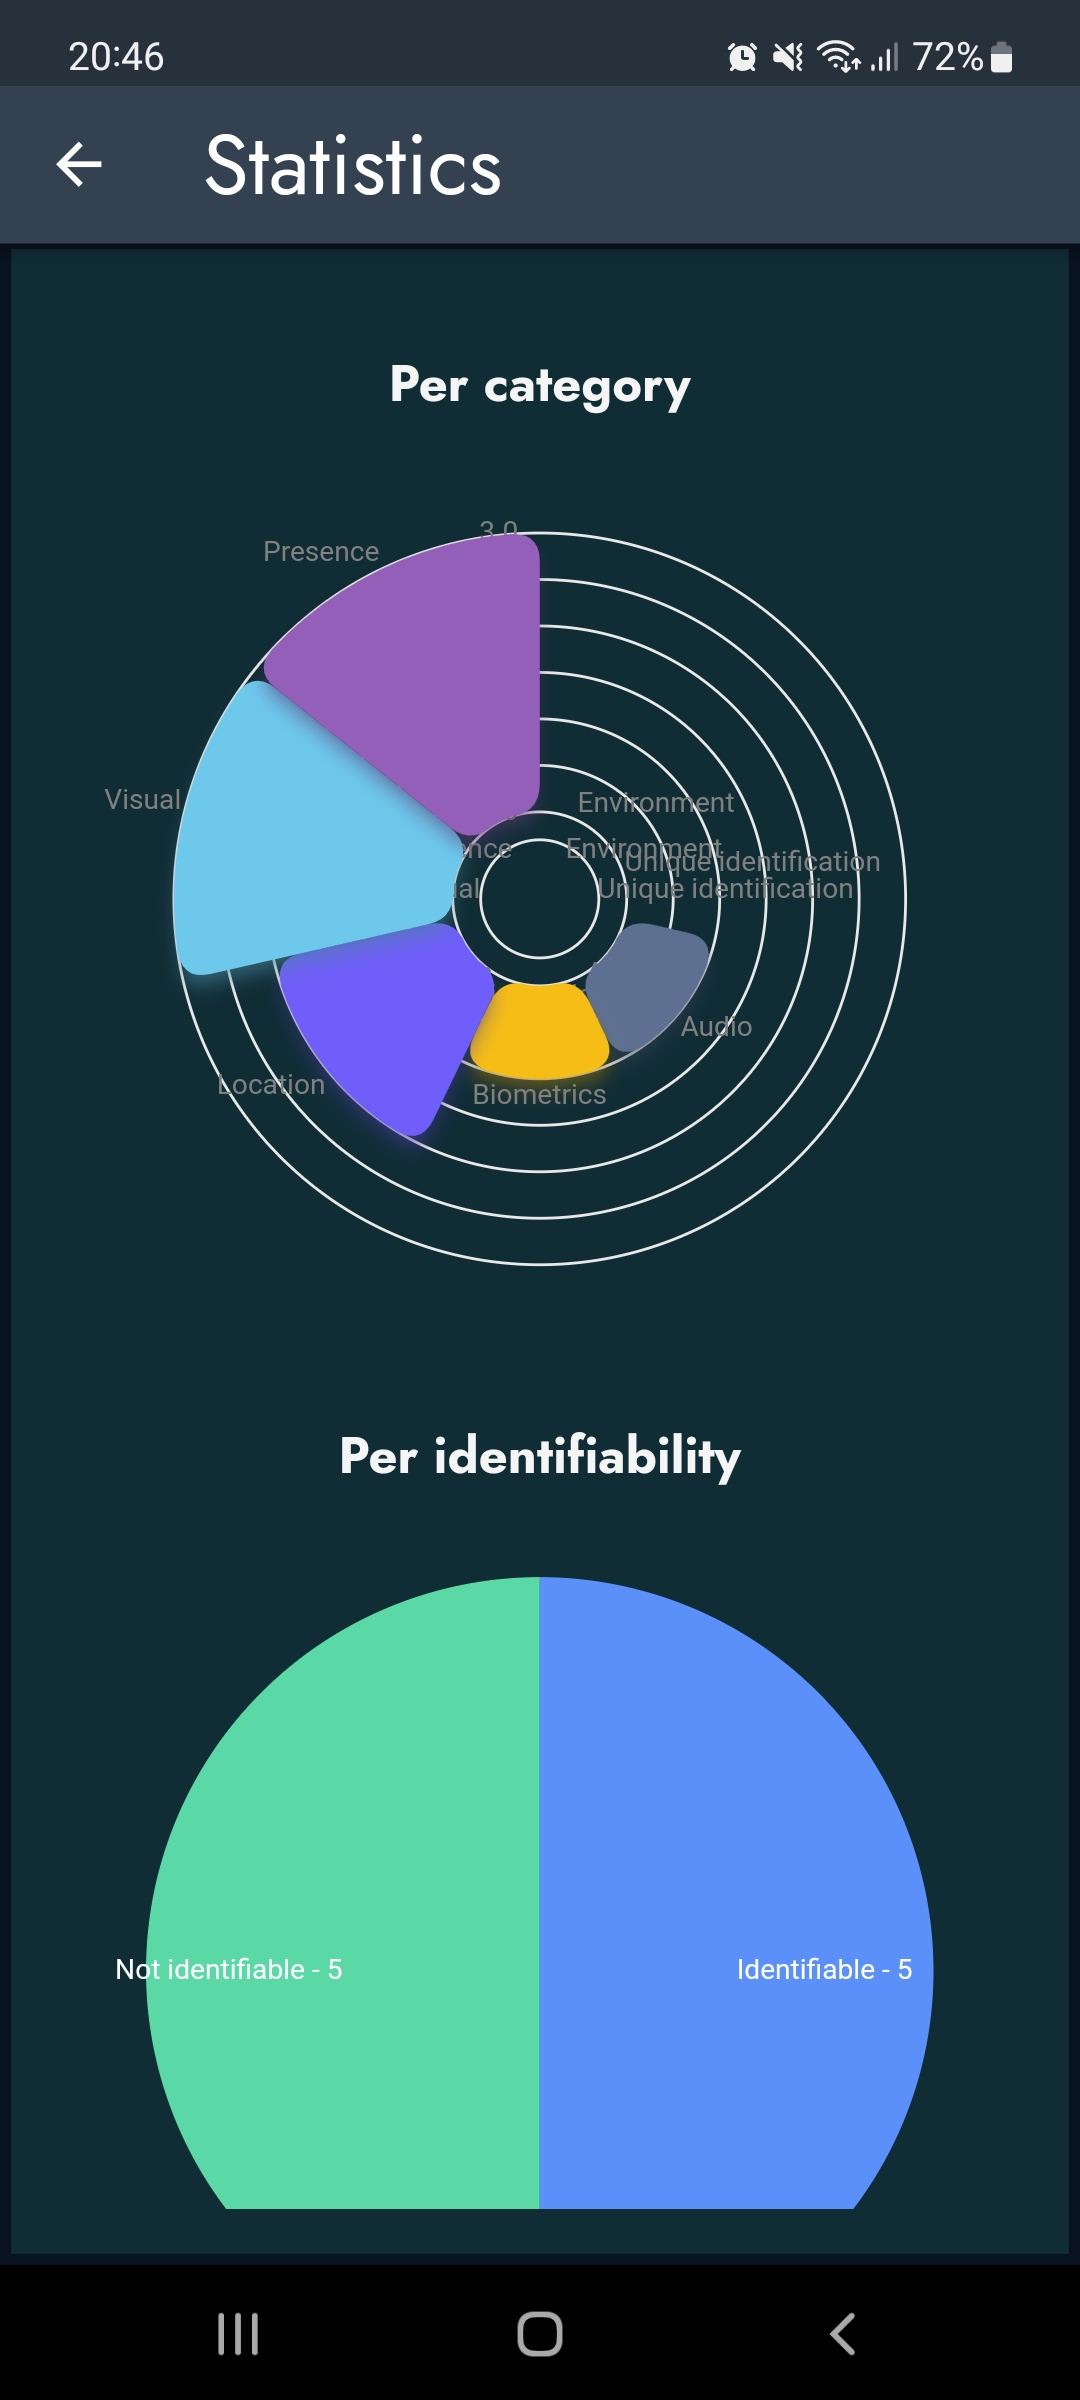
\includegraphics[width=125pt]{../assets/images/live_statistics.jpg}
        \caption{}
        \label{fig:live_statistics}
    \end{subfigure}
    \caption{Live version of the application with pages: (a) homepage, (b) about, (c) FAQ, (d) devices, (e) device information and (f) statistics pages.}
    \label{fig:live_app}
\end{figure}

\subsection{Development}

As was defined in the system requirements specification, the Flutter
framework was the development tool used for the reasons described.
This allows for the relatively fast development of an application for
mobile without using native tools, which would significantly lengthen the
development time.

Figure \ref{fig:dbmodel} shows an entity relationship diagram, this type of
diagram is usually created for relational databases, but, as is the case of
Firestore, the database used is document-oriented, or NoSQL. This differs from
relational databases in that data is stored in an object rather than in separate
tables with relationships between them, but it can work identically to a relational
database if configured properly. One of the main reasons to use Firestore is that
it has great integration with Flutter. There are only three documents used to
store backend data, one for IoT devices, one for users and another for categories.
A document for users is used to extend Firebase Authentication, which can only
store the email and password of users and also be used for email confirmation.

\begin{figure}[H]
    \centering
    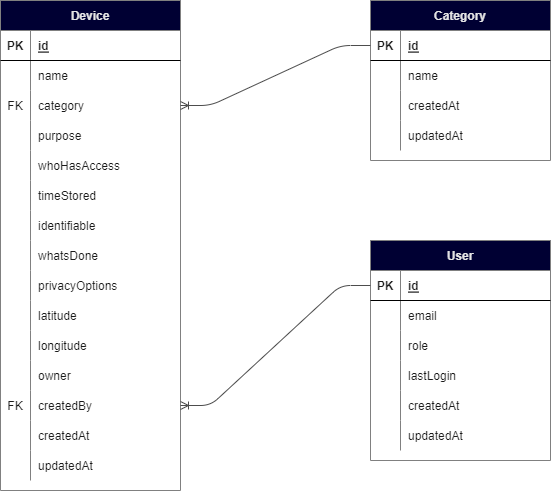
\includegraphics[width=340pt]{../assets/images/erdiagram.png}
    \caption{Entity relationship diagram of database.}
    \label{fig:dbmodel}
\end{figure}

The development phase of this work took the greatest amount of time,
it started almost after carrying out the requirements assessment, while
the prototypes were being created and continued after conducting the
usability tests. It will still be continued to be developed even after
the production version 1.0 is released.

What makes it take so much time is due to the resolution of bugs and
problems that appear during the normal course of development. Using
the Firestore database proved to be somewhat difficult because
it is not as intuitive to create queries between different objects
as it is using the SQL language.

Users can, when they start the application for the first time, freely use it to see
which devices are in their vicinity,
information about the devices, information about the application itself, and
information about privacy in general and more specifically privacy in IoT systems
which they can use to improve their digital literacy. What they cannot do is
add a new device to the application or edit a device's information. The user has
to create an account first to do these operations. The decision to add an
account creation before the user can add or edit a device is to prevent
bad actors to add bogus data to the application making unusable for the majority
of people, this solution does not completely solve this issue (because bad actors
can still create an account and add bogus data anyway) but it helps to slow
down the insertion of bad data.

Upon account creation the only data entry that can be considered sensitive that
the user has to input is an email address.
After the user has created an account and logs in, the user can add devices to the application with the following information:

\begin{itemize}
    \item[$\bullet$]
    The \textbf{name of the device}: This serves to differentiate between the various devices on the application and as such should be unique to each device, it is used on various routes and is one of the first fields that users see about a device. A single device does not have an \textit{official} name, what is more probable is that the device has a model name or is part of a system with its own name. The user creates the name, this could be abused by bad actors but it is extremely discouraged. It is used for aesthetic reasons.
    \item[$\bullet$]
    The \textbf{category of the device}: This is used to categorize each devices main type of information that the device is collecting. These can be of the following:
    \begin{itemize}
        \item[$\circ$] \textbf{Visual}: The device mainly collects visual information with maybe a video camera.
        \item[$\circ$] \textbf{Audio}: The device mainly collects audio information with a sound recorder.
        \item[$\circ$] \textbf{Presence}: The device can detect the presence of nearby objects or persons. This is not the same as the location category because the device does not know the location of an individual, it merely knows that the individual is nearby. These type of devices can be used, for example, to collect information about how many people frequent a specific store.
        \item[$\circ$] \textbf{Location}: The device can detect the exact or approximate location of an individual, it can use GPS to get this kind of information.
        \item[$\circ$] \textbf{Biometrics}: The devices collects biometric data, this can be the number of steps an individual (or animal) takes, or health related data like the heart beat.
        \item[$\circ$] \textbf{Environment}: These type of devices collect environmental data, they can be used for agriculture or weather forecasting by collecting, for example, temperature, humidity or wind speed/direction data.
        \item[$\circ$] \textbf{Unique identification}: This category is for a device that can uniquely identify an individual, the device itself most likely is not capable of doing it but with other information that the device has access to, it can be used to cross reference of information and as such uniquely identify a person. An example of this would be a device a device that can collect visual data and with facial recognition used against other data in a database it can uniquely identify an individual.
    \end{itemize}
    \item[$\bullet$]
    The \textbf{purpose for the data collection}: Defines what is the purpose for the collection of the data, if a device collects temperature and humidity data and is used by a weather based company or government agency then the purpose for the data collection is for weather forecasting.
    \item[$\bullet$]
    \textbf{Who has access to the collected data}: Disclose an individual or group of individuals that have access to the data of the device, if the device is part of a closed system it can be that only an individual as access to the data but most likely various groups of people have access to the data, some with more data than others depending on the permissions they have. If the device publicizes its data then everyone has access to it.
    \item[$\bullet$]
    \textbf{For how long is the data stored}: Pinpoint the duration of the stored data in the device or system, due to legislation passed in various countries this duration has a limit, in some cases the data cannot be stored for more than one year.
    \item[$\bullet$]
    \textbf{Can the data identify anyone}: Used to quickly identify if a particular device can identify an individual or not. If the device belongs to the ``Unique identification'' category then this should be active.
    \item[$\bullet$]
    \textbf{What is being done with the data}: This could be assumed to be similar to the \textbf{purpose} field mentioned above but it should be used to diagnose what is being done now with the data collected, in certain situations it might coincide with the purpose for the data collection.
    \item[$\bullet$]
    \textbf{Privacy options}: The user can insert an url for the device's privacy options, in some cases the device, or company, has a website with information on privacy options, or privacy policy. If the device uses a mobile application then a link to the this application can be inserted here.
    \item[$\bullet$]
    \textbf{Coordinates of the device}: Used to express the latitude and longitude of the device so that it can be shown on the map, on the homepage of the application.
    \item[$\bullet$]
    \textbf{Who owns the device}: Who is the device owner, if it belongs to an organization then the name of the organization should appear here otherwise if the device belongs to a person then the person's name should \textbf{not} appear, it should say private or something similar.
\end{itemize}

The user is not required to provide information to satisfy all items on this list, the
only information that is required in order to add a device to the application is
the name, category and coordinates of the device, all other
information is optional but should be provided for the sake of guaranteeing a good
experience to other users of the application. The information provided
should be verified by the user beforehand so that bogus data does not clutter
the application, in this case there are no absolute ways of guaranteeing this
but the maintainer of the application edit wrong information or in some
cases remove it, other users can also edit any device data. This is an
open platform so it is expected that users act in good faith.

The usability tests were crucial to the development of the application,
they improved significantly the user experience along with changes to the
user interface.

Usability tests were conducted in person with 7 participants of different
ages, professional fields and qualifications. The participants' ages range
from 40 to 50 on average, their professional backgrounds include accounting,
management, social services and agriculture, and their academic qualifications range from
basic education to bachelor's degree. Unlike the dissemination of the questionnaire,
participants for these tests were recruited informally. Before doing the tests,
some questions were made to evaluate the general level of digital literacy
regarding IoT and privacy, then the participants were asked to fill in the
survey, if they had not done it yet, as this gives some insight into what the
application is about. The usability tests consisted of single ease
questions \cite{tedesco2006comparison}
and the system usability scale \cite{brooke1996sus}, as can be seen on \nameref{appendix:usability_tests}.
The single ease questions were used after the participant performed each task, the
participant would answer how difficult they though the task was in a
scale from 1 to 7. The system usability scale was used after the participants
performed all tasks, with the same type of scale.
